\glsresetall

\section{Advancing our understanding of the human microbiome using QIIME}\label{section_book}

High-throughput DNA sequencing technologies, coupled with advanced bioinformatics
tools, have enabled rapid advances in microbial ecology and our understanding of
the human microbiome. \gls{qiime} is an open-source bioinformatics software package
designed for microbial community analysis based on DNA sequence data, which provides
a single analysis framework for analysis of raw sequence data through publication
quality statistical analyses and interactive visualizations. In this paper, we
demonstrate the use of the \gls{qiime} pipeline to analyze microbial communities
obtained from several sites on the bodies of transgenic and wild-type mice, as
assessed using 16S \gls{rrna} gene sequences generated on the Illumina MiSeq
platform. We present our recommended pipeline for performing microbial community
analysis, and provide guidelines for making critical choices in the process. We
present examples of some of the types of analyses that are enabled by \gls{qiime},
and discuss how other tools, such as phyloseq and R, can be applied to expand upon these analyses.

\subsection{Introduction}

Advances in DNA sequencing technologies, together with the availability of culture-independent
sequencing methods and software for analyzing the massive quantities of data resulting from
these technologies, have vastly improved our ability to characterize microbial communities in
many diverse environments. The human microbiota, the collection of microbes living in or on the
human body, is of considerable interest: microbial cells outnumber human cells in our bodies by
a ratio of up to 10 to 1 \cite{Savage1977}. These microbial communities contribute to healthy
human physiology \cite{DeFilippo2010, Dethlefsen2011, Spencer2011} and development
\cite{Dominguez-Bello2010, Koenig2011}, and dysbiosis (or imbalance in these communities) is now
known to be associated with disease, including obesity \cite{Turnbaugh2009Core} and Crohn's disease
\cite{Eckburg2007}. More recently, evidence from transplants into germ-free mice suggests that
some of these associations may be causal, because certain phenotypes can be transmitted by
transmitting the microbiota \cite{Carvalho2012, McLean2012, Turnbaugh2009}, even including
transmission of human phenotypes into mice \cite{Heijtz2011, Koren2012, Smith2013}.

Illumina's MiSeq and HiSeq DNA sequencing instruments respectively sequence tens of millions,
or billions, of DNA fragments in a single sequencing run \cite{Kuczynski2011}. The rapidly
increasing data volumes typical of recent studies drives a need for more efficient and scalable
tools to study the human microbiome \cite{Gonzalez2012}. \gls{qiime} \cite{Caporaso2010} is an
open-source pipeline designed to provide self-contained microbial community analyses, from interacting
with raw sequence data through publication-quality statistical analyses and visualizations.

\gls{qiime} integrates commonly used third-party tools, and implements many diversity metrics,
statistical methods, and visualization tools for analyzing microbial data. Consequently, most
individual steps in the microbial community analysis can be performed in multiple ways. Here, we
describe how samples are prepared for an Illumina MiSeq run, the \gls{qiime} pipeline, and our
view of the current best practices for analyzing microbial communities with \gls{qiime}. Although
there are other pipelines available, including mothur \cite{Schloss2009}, the RDP
tools \cite{Olsen1991, Olsen1992}, ARB \cite{Ludwig2004}, \gls{vamps} \footnote{\label{vampsurls}\url{http://vamps.mbl.edu}},
and other platforms, in this review we focus on analysis with the MiSeq platform and \gls{qiime}
as this combination is increasingly popular as a method for analyzing microbial communities and
a detailed comparison of other available pipelines and sequencing platforms is beyond the
scope of the present work.

\subsection{QIIME as integrated pipeline of third party tools}

An early barrier to adoption of \gls{qiime} was that it was difficult to install,
in part because of the large number of software dependencies (third party packages
that need to be installed before \gls{qiime} is operational). The large number of
dependencies was, however, a deliberate choice made during \gls{qiime} development.
To build a pipeline for sequence analysis that encompasses the many steps from sequence
collection, curation, and statistical analysis, the user must consider many existing
tools that have been developed to perform specific functions, and extensively benchmarked
on their ability to perform these functions, such as the UCLUST program for clustering
sequences into \gls{otu} \cite{Edgar2010}. A pipeline thus has two options: either
re-implement the algorithm, or use the existing software (by creating a “wrapper”
that allows its input and output to be incorporated into the pipeline). The \gls{qiime}
developers choose to wrap all the algorithms rather than re-implement them. This choice
preserves the integrity of the programs that make up the pipeline, as there is no doubt
that the tool being used is the one designed, created, and tested by the original authors,
and, in most cases, peer-reviewed by the scientific community. The reuse of existing
software also allows the \gls{qiime} pipeline to include and distribute newly developed
and improved algorithms more rapidly than would be possible if each algorithm had to be
re-implemented and re-tested to check that it matched the original. Thus \gls{qiime} users
can be sure that they have the most up-to-date tools for their analysis, and can credit the
authors of the component software packages appropriately.

One important, but sometimes poorly understood, aspect of the \gls{qiime} pipeline is that
it wraps algorithms and tools produced by other researchers into a single pipeline for
sequence analysis. It is therefore important to cite the individual tools that you use as well
as \gls{qiime} itself. For example, an analysis using the default \gls{qiime} parameters \cite{Caporaso2010}
would use UCLUST \cite{Edgar2010} to cluster the sequences against the GreenGenes
database \cite{DeSantis2006}, assign taxonomy using the RDP classifier \cite{Wang2007}, and
build \gls{pcoa} beta diversity plots using UniFrac \cite{Lozupone2005}. It is important for
researchers who are considering contributing to the \gls{qiime} pipeline to recognize
that their contributions will be cited, so that they can continue to expand upon their work.
For example, the pick\_otus.py script alone offers a choice of nine different clustering algorithms,
each developed by researchers who should be acknowledged if their particular algorithm is used.

For taxonomy databases and other reference databases, including GreenGenes, it is also
important to cite the release version that you are using \cite{DeSantis2006}, not least
because the results will change depending on which release you used, and others may not
be able to reproduce your results without this information. For GreenGenes, the default
taxonomy database in \gls{qiime}, the version is named after the release date, such as
the 12\_10 release. The latest version of GreenGenes can always be downloaded from the
qiime.org website. Using the same GreenGenes reference database version is critical for
comparisons of taxonomy assignments and \gls{otu} across different studies. For this
reason, all the studies in the \gls{qiime} database are always processed against the
same release version of GreenGenes.

An overview of some of the key tools used by the default \gls{qiime} pipeline follows:

\begin{itemize}
    \item UCLUST \cite{Edgar2010}. Used for \gls{otu} picking.
    \item USEARCH \cite{Edgar2010}. Used for \gls{otu} picking and chimera checking.
    \item RDP Classifier \cite{Wang2007}. Used for taxonomy assignment.
    \item GreenGenes Database \cite{DeSantis2006}. Used as a reference database for taxonomy assignment and reference-based \gls{otu} picking (see below).
    \item PyNAST \cite{Caporaso2010PyNAST}. Used for multiple sequence alignment.
    \item UniFrac \cite{Lozupone2005}. Used as a phylogenetic metric for beta diversity analysis.
\end{itemize}

\subsection{PCR and sequencing on Illumina MiSeq}

Microbial community analysis typically begins with the extraction of DNA from primary
samples (note that although most of this DNA comes from cells in the sample, some may
consist of dead cells or extracellular DNA, so the representation of the active community
from these sources is not perfect). Although methods for DNA extraction vary, several
large initiatives such as the \gls{emp} \cite{Gilbert2010} and the \gls{hmp}
\cite{TheHumanMicrobiomeProjectConsortium2012, Consortium2012, Turnbaugh2007} have
standardized on the MOBIO PowerSoil DNA extraction kit \footnote{\url{http://www.mobio.com}}
to efficiently recover DNA from a wide range of sample types. After extraction, samples are
\gls{pcr} amplified under permissive conditions with primers containing the MiSeq sequencing
adapters, a 12-nucleotide Golay barcode (first introduced in \cite{Fierer2008}) on the forward
primer, followed by the bases matching the 16S \gls{rrna} gene; the reverse primer is not
barcoded \cite{Caporaso2012}. The annealing temperature is set to 50$^{\circ}$C, which in our
hands minimizes \gls{pcr} artifacts (both primer dimer and background ‘smear’) while encouraging
the primers to anneal to the largest diversity of sequences possible. Similarly, we believe that
including sequencing adaptors and barcodes in the \gls{pcr} step has advantages over multiple
enzymatic treatments of the 16S amplicon that are otherwise needed to introduce adaptors and
barcodes after \gls{pcr}. The first, and most important consideration is the reduction of sample
handling, which lowers the chance of contamination, mislabeling and loss of small-volume samples
during preparation. Combining the adapters and barcodes in the \gls{pcr} step allows for exact
well-to-well mapping of samples to primers, providing a standardized way to track sample-barcode
combinations through library preparation, an important consideration when sequencing hundreds to
thousands of samples using 96- or 384-well sample preparation formats.

Because the MiSeq can generate a large number of sequences per run, many samples can be multiplexed
on each single sequencing run. The choice of barcodes thus deserves some attention. For instance,
homebrew ‘barcodes’ can be as simple as using an arbitrary sequence of known nucleotides placed at
the front of the amplicon and fed into an informatics pipeline for detection. Although simple, this
approach has limited ability to detect sequencing error \cite{Caporaso2012}, and increases the risk
of misassignment of a sequence to the wrong sample. The use of error correcting barcodes, such as
Hamming \cite{Hamady2008} or Golay codes \cite{Caporaso2012}, allows the user to detect and correct
errors in the barcode, decreasing the chances that a sequence is assigned to the wrong sample.
Error-correcting barcodes also allow the user to retain more sequences, because 8-nucleotide Hamming
codes can detect and correct 2 and 1 bit errors, respectively \cite{Hamady2008}, and 12-nucleotide
Golay codes can detect and correct 4 and 3 bit errors, respectively \cite{Hamady2009}. With the
unique Golay codes described in \cite{Caporaso2012}, up to 2167 samples could be multiplexed on a
single MiSeq run at a depth of 4600 per sample, certainly sufficient to detect the effects of many
biological phenomena of interest \cite{Kuczynski2010, Kuczynski2010Patterns}. As the \gls{qiime}
default settings detect Golay barcodes, we encourage the use of these codes when possible to maximize
sequence retention and assignment accuracy.

Detailed instructions for loading the MiSeq for amplicon runs with custom barcodes can be found on
the \gls{emp} website \footnote{\url{http://www.earthmicrobiome.org}}. Briefly, pooled libraries are
analyzed by Bioanalyzer (Agilent Technologies) and diluted to 2 $\mu M$ quantitated by use of a
Qubit Fluorometer (Life Technologies, High Sensitivity reagents). The phiX spike-in library
(Illumina Inc.) is also diluted to 2 $\mu M$ prior to use. Denaturation of the pooled 16S \gls{rrna}
gene amplicon libraries and the phiX control is performed according to manufacturer's
instructions (Illumina Inc.), giving a denatured template concentration of 20 $\rho M$. Denatured
templates are further diluted to 5 $\rho M$ (using Illumina HT1 buffer) and subsequently combined to
give an 85\% 16S \gls{rrna} gene amplicon library and 15\% phiX control pool (1000 $\mu L$ total volume).
Improvements in the Illumina analysis software may allow reduction of this phiX spike-in, allowing more
of the sequences to be used for 16S \gls{rrna} gene amplicons.

MiSeq reagent cartridges are prepared according to the manufacturer's instructions (Illumina Inc.).
The sample pool (1000 $\mu L$ total volume) is loaded in to cartridge position 17. Custom 16S \gls{rrna}
gene Read 1, Index Read, and Read 2 sequencing primers are added directly to cartridge wells containing
the standard Illumina Read 1, Index Read, and Read 2 sequencing primers (wells 12, 13 and 14 respectively,
5 $\mu L$ each primer at 100 $\mu M$ concentration \cite{Caporaso2012}). Primers are added to wells using
a long gel loading tip, and gently mixed using a plastic Pasteur pipette. Care must be taken to assure that
reagents in the cartridge are localized to the bottom of the wells, and that no bubbles are present.

The spike-in of PhiX, at least at low levels, is still critical for obtaining usable amplicon data because
the optics require diversity at each nucleotide position, which is not possible with absolutely conserved
nucleotides within the 16S \gls{rrna} gene (or most other genes of interest). Many users have had difficulty
mixing this protocol for custom amplicons with Illumina's own indexing protocol, which allows a maximum of
96 samples to be multiplexed per run at the time of writing. It is critical to use either this protocol exactly
(allowing arbitrary numbers of custom barcodes) or to use Illumina's barcoding protocol, but not to mix and
match steps and reagents.

\subsection{QIIME workflow for conducting microbial community analysis}

The Illumina MiSeq technology can generate up to 107 sequences in a single run \cite{Kuczynski2011}.
\gls{qiime} takes the instrument output, and generates useful information about the community represented
in each sample. At a coarse-grained level, we divide this process into “upstream” and “downstream” stages
(Figure ~\ref{BFigure1}). The upstream step includes all the processing of the raw data (sequencing output),
and generating the key files (\gls{otu} table and phylogenetic tree) for microbial analysis. The downstream
step uses the \gls{otu} table and phylogenetic tree generated in the upstream step to perform diversity
analysis, statistics and interactive visualizations of the data. Additionally, \gls{qiime} increasingly
interfaces with other packages such as IPython and R, allowing additional analyses to be conducted.

\begin{figure}[htbp]
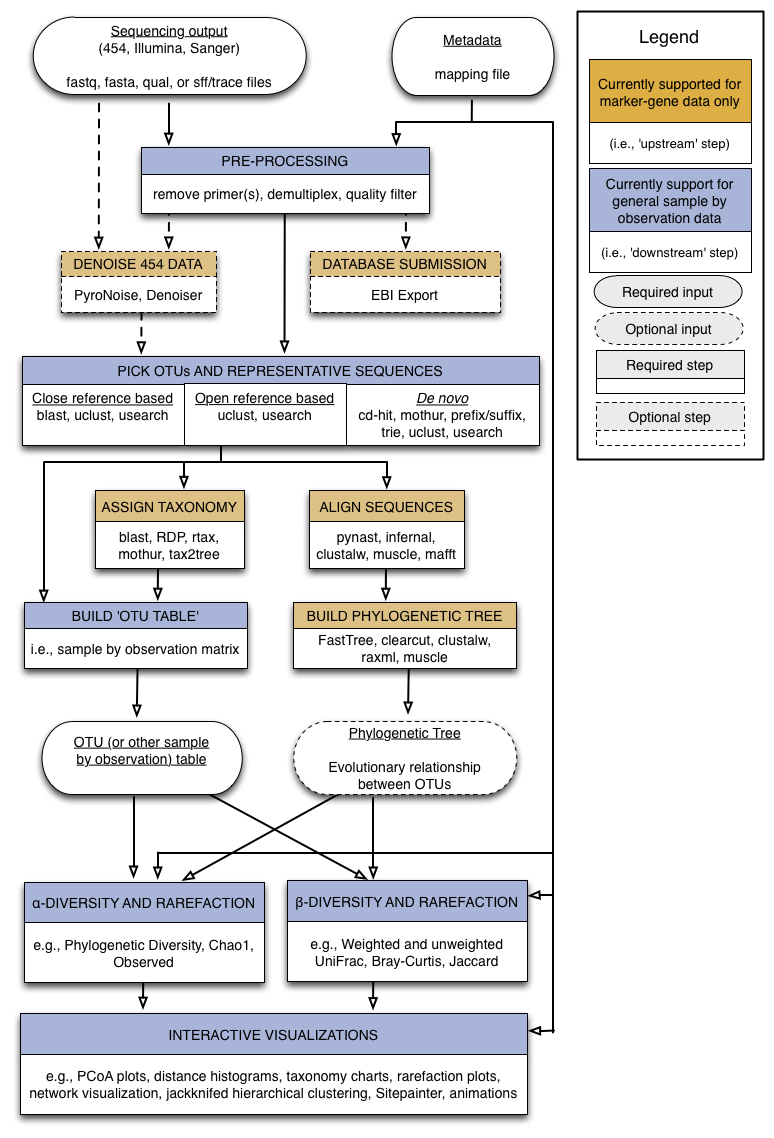
\includegraphics[width=0.75\columnwidth]{chapter_book_figures/Figure_1.jpg}
\caption[\gls{qiime} workflow overview]{\textbf{\gls{qiime} workflow overview.} The Upstream process (brown boxes)
includes all the steps that generate the \gls{otu} table and the phylogenetic tree. This step starts by
preprocessing the sequence reads and ends by building the \gls{otu} table and the phylogenetic tree.
The Downstream process (blue boxes) includes steps involved in analysis and interpretation of the results,
starting with the \gls{otu} table and the phylogenetic tree and ending with alpha and beta diversity analyses,
visualizations and statistics.}
\label{BFigure1}
\end{figure}

To illustrate some of the main features of \gls{qiime}, together with some of the analyses that can be
performed outside \gls{qiime}, we use an example dataset consisting of samples from different body sites
of 12 mice: the oral cavity, ileum, cecum, colon, fecal pellet, skin and whole mouse sample by homogenizing
the mouse carcass. 7 mice were wild type genotype (WT from here so on), while the 5 remaining mice were
transgenic (TG from here so on). The samples were collected by students during the IQ-Bio course taught by
Manuel Lladser and Rob Knight during Spring 2013 at University of Colorado at Boulder (course identifiers:
APPM5720-001-2013, CHEM4751-001-2013, CHEM5751-001-2013, CSCI4830-006-2013, CSCI7000-006-2013, MCDB6440-001-2013).

\subsubsection{Upstream analysis steps}

The \gls{qiime} analysis workflow starts with the sequencing output (fastq files), and a user-generated
mapping file. The mapping file contains information for understanding what is in each sample and is
therefore critical for performing the rest of the analyses; it is in tab-delimited text format. The main
information in this file is a unique identifier for each sample, the barcode used for each sample, the primer
sequence used, and a description for each sample, together with additional user-defined information that is
necessary for understanding the results such as which species the sample was taken from, which site on the
body is being studied, clinical variables relevant to the study, etc. The sample identifier, barcode and
primer sequence information are required for the first step of the \gls{qiime} workflow. This preprocessing
step combines sample demultiplexing, primer removal and quality-filtering. Additional information provided
about the samples in the mapping file is helpful for later steps, especially for analyses that aggregate
the samples by these fields (for example, comparing lean to obese subjects). We therefore recommend
including as much additional data about the samples as possible (often called “sample metadata”). This
auxiliary information is also very useful for identifying contaminated samples. For example,
SourceTracker \cite{Knights2011} is a package included in \gls{qiime} that identifies the proportion
of different community sources, including contamination, in each sample based on a database of samples
from known communities.

\textbf{De-multiplexing and quality filtering.} As mentioned above, high-throughput sequencing allows
multiple samples to be combined in a single sequencing run \cite{Kuczynski2011}. However, each sequence
must then be linked back to the individual sample that it came from via a DNA barcode. The barcodes,
which are short DNA sequences unique to each sample, are incorporated into each sequence from a given
sample during PCR. \gls{qiime} uses the barcodes in the mapping file to demultiplex, i.e. to assign the
sequences back to the samples they are derived from, using error-correcting codes where available
(as noted above). \gls{qiime} is also able to demultiplex variable-length barcodes such as those used in
the \gls{hmp}: see Variable-length barcodes in Other features below.

During demultiplexing, \gls{qiime} removes the barcodes and primer sequences because they are not needed
in later steps. Thus, the result after demultiplexing is a sequence matching the amplified 16S \gls{rrna} gene.

The third part of preprocessing is quality-filtering. Quality-filtering improves diversity estimates with
Illumina sequencing substantially \cite{Bokulich2013}. Illumina instruments, like most sequencing instruments,
generate a quality score for each nucleotide (Phred), related to the probability that each nucleotide was
read incorrectly. \gls{qiime} uses the Phred score and user-defined parameters to remove sequence reads
that do not meet the desired quality. These user-defined parameters are: the percentage of consecutive
high quality base calls ($p$), the maximum number of consecutive low quality base calls ($r$), the
maximum number of ambiguous bases (typically coded as N) ($n$) and the minimum Phred quality score ($q$).
For a detailed discussion of how these parameters affect diversity results, see \cite{Bokulich2013}.
This study recommends standard values for these parameters as $r = 3$, $p = 75\%$, $q = 3$ and $n = 0$,
which are the default values in the \gls{qiime} pipeline. However, the optimal values for these parameters
can vary both for individual sequencing runs and for different downstream analyses: for example,
analyses such as machine learning benefit from larger numbers of low-quality sequences, whereas accurate
counts of \gls{otu}s from a mock community require fewer, higher-quality sequences. Table~\ref{btable1} contains
an overview of the guidelines presented in \cite{Bokulich2013} for tuning these parameters to a given dataset.


\begin{sidewaystable}[htbp]
\centering
\caption[Overview of the guidelines to tune up the quality filtering parameters (adapted from \cite{Bokulich2013})]{Overview of the guidelines to tune up the quality filtering parameters.}\label{btable1}
\begin{tabular*}{\textwidth}{ccccc}
\toprule
Dataset characteristics & q & p & r & Results\\
\midrule
Majority of high-quality, & \multirow{2}{*}{increase} & \multirow{2}{*}{increase} & \multirow{2}{*}{-} & Retrieving full-length sequences with low error rates,\\
full-length sequences & & & & increasing the discovery rate of rare \gls{otu}s\\
\midrule
Short reads, or reads truncated & \multirow{2}{*}{-} & \multirow{2}{*}{lower} & \multirow{2}{*}{increase} & Retain lower-quality but\\
by early low-quality base calls & & & & taxonomic usefult reads\\
\midrule
Maximize read count for machine- & \multirow{3}{*}{-} & \multirow{3}{*}{lower} & \multirow{3}{*}{-} & \multirow{3}{*}{Increased sample size}\\
learning tools, cross-metadata & & & & \\
\gls{otu} counts comparison, etc & & & & \\
\bottomrule
\end{tabular*}
\end{sidewaystable}

The Illumina quality filtering approach differs in its fundamental principles from
454 denoising \cite{Quince2009, Reeder2010}. 454 denoising is based on flowgram
clustering \cite{Quince2009, Quince2011} and is primarily targeted at reducing
homopolymer runs, which are not a problem on the Illumina platform to the same extent.
In contrast, the Illumina quality filtering is based on a per-base Phred quality score
and does not target indels.

The \gls{qiime} quality filtering process works as follows. Starting at the
beginning of the sequence, \gls{qiime} checks that the next $r$ Phred values exceed
the user-defined quality threshold $q$. If the test is positive, it continues
slicing the window of $r$ bases until the test fails, or the end of the sequence
is reached. The sequence is then trimmed to the last base that met the quality
threshold. The next test determines whether the length of the trimmed sequence
exceeds $p$, expressed as the percentage of length of the raw sequence. If this
check fails, the sequence is excluded. Otherwise, \gls{qiime} performs the last
check on the sequence, which counts the number of ambiguous characters (N) in the
trimmed sequence and checks that it is less than $n$. If the test fails, the
sequence is rejected. \gls{qiime} combines the de-multiplexing, primer removal and
quality filtering processes in a single script, split\_libraries\_fastq.py:

\begin{lstlisting}[language=bash]
split_libraries_fastq.py
  -i $PWD/IQ_Bio_16sV4_L001_sequences.fastq.gz \
  -b $PWD/IQ_Bio_16sV4_L001_sequences_barcodes.fastq.gz \
  -m $PWD/IQ_Bio_16sV4_L001_map.txt -o $PWD/slout \
  --rev_comp_mapping_barcodes
\end{lstlisting}

In our example dataset, we used the --rev\_comp\_mapping\_barcodes option in order
to indicate that the barcodes present in the mapping file are reverse complements of
Golay 12 barcodes. We used the recommended default parameters for quality filtering
on this dataset. However, to change the values for the $r$, $p$, $n$ and $q$ quality
filtering parameters, we can use the $-r$, $-p$, $-n$ and $-q$ options to the script.
This command will write a FASTA-formatted file in the slout folder, called seqs.fna,
which contains the demultiplexed sequences that pass the quality filter. Each sequence
contains the information about which sample it came from encoded in the name of the sequence.

Multiple lanes of Illumina fastq data can be processed together in a single call
to the script, just by passing the sequence files, the barcode files and the mapping
files in the same order to the $-i$, $-b$ and $-m$ options, respectively. For example,
with two lanes, the command would look like:

\begin{lstlisting}[language=bash]
split_libraries_fastq.py
  -i sequences1.fastq,sequences2.fastq
  -b sequences1_barcodes.fastq,sequences2_barcodes.fastq
  -m mapping1.txt,mapping2.txt -o slout
\end{lstlisting}

The user can check how many sequences have been demultiplexed and passed quality-filtering
by using the count\_seqs.py command. This command also shows the mean and standard
deviation of the sequence length:

\begin{lstlisting}[language=bash]
count_seqs.py -i $PWD/slout/seqs.fna

12687021 :slout/seqs.fna (Sequence lengths (mean +/- std):
150.9989 +/- 0.1715)

12687021 : Total
\end{lstlisting}

\textbf{\gls{otu} picking.} The next step is clustering the preprocessed sequences
into \gls{otu}, which in traditional taxonomy represent groups of organisms defined by
intrinsic phenotypic similarity that constitute candidate taxa \cite{Sneath1973, Sokal1963}.
For DNA sequence data, these clusters, and hence the \gls{otu}s, are formed based on sequence
identity. In other words, sequences are clustered together if they are more similar than a
user-defined identity threshold, presented as a percentage ($s$). This level of threshold
is traditionally set at 97\% of sequence similarity, conventionally assumed to represent
bacterial species \cite{Drancourt2000}; other levels approximately represent other taxa,
although the fit between molecular data and traditional taxonomy varies for different taxa.
\gls{qiime} supports three approaches for \gls{otu} picking (de novo, closed-reference and open-reference),
and multiple algorithms for each of these approaches (Table ~\ref{btable2}). The de novo
approach (Figure ~\ref{bfigure2}a) groups sequences based on sequence identity. The closed-reference approach
(Figure ~\ref{bfigure2}b) matches sequences to an existing database of reference sequences. If a sequence fails
to match the database, it is discarded. The open-reference approach (Figure ~\ref{bfigure2}c) also
starts with an existing database and tries to match the sequences against them. However, if a
sequence does not match the database, it is added to the database as a new reference sequence.

\begin{sidewaystable}[htbp]
\centering
\caption[Supported \gls{otu} picking methods in \gls{qiime}, with a brief description of the algorithm employed and in which \gls{otu} picking approach can be used.]{Supported \gls{otu} picking methods in \gls{qiime}, with a brief description of the algorithm employed and in which \gls{otu} picking approach can be used.}\label{btable2}
\renewcommand{\arraystretch}{0.6}% Tighter
\begin{tabular*}{\textwidth}{cccccc}
\toprule
Method & \multicolumn{3}{c}{Picking approach} & Description & Reference \\
\midrule
& de & closed & open & & \\
& novo & reference & reference & & \\
\midrule
\multirow{2}{*}{cd-hit} & \multirow{2}{*}{Yes} & \multirow{2}{*}{-} & \multirow{2}{*}{-} & Applies a "longest-sequence-first list & \multirow{2}{*}{\cite{Li2006, Li2001}}\\
& & & & removal algorithm" to cluster sequences & \\
\midrule
\multirow{3}{*}{Mothur} & \multirow{3}{*}{Yes} & \multirow{3}{*}{-} & \multirow{3}{*}{-} & Takes an aligned set of sequences and clusters & \multirow{3}{*}{\cite{Schloss2009}}\\
& & & & them using a nearest-neighbor, furthest-neighbor & \\
& & & & or average-neighbor algorithm. & \\
\midrule
\multirow{2}{*}{prefix/suffix} & \multirow{2}{*}{Yes} & \multirow{2}{*}{-} & \multirow{2}{*}{-} & Clusters sequences which are identical & \multirow{2}{*}{\gls{qiime} team, unpublished}\\
& & & & in their first and/or last bases. & \\
\midrule
\multirow{3}{*}{Trie} & \multirow{3}{*}{Yes} & \multirow{3}{*}{-} & \multirow{3}{*}{-} & Clusters sequences which are identical sequences & \multirow{3}{*}{\gls{qiime} team, unpublished}\\
& & & & and sequences which are subsequences & \\
& & & & of other sequences. & \\
\midrule
\multirow{2}{*}{blast} & \multirow{2}{*}{-} & \multirow{2}{*}{Yes} & \multirow{2}{*}{-} & Compares and clusters each sequence against & \multirow{2}{*}{\cite{Altschul1990}}\\
& & & & a reference database of sequences. & \\
\midrule
\multirow{2}{*}{uclust} & \multirow{2}{*}{Yes} & \multirow{2}{*}{Yes} & \multirow{2}{*}{Yes} & Creates seed sequences which generate & \multirow{2}{*}{\cite{Edgar2010}}\\
& & & & clusters based on percent identity. & \\
\midrule
\multirow{4}{*}{usearch} & \multirow{4}{*}{Yes} & \multirow{4}{*}{Yes} & \multirow{4}{*}{Yes} & Creates seed sequences which generate & \multirow{4}{*}{\cite{Edgar2010}}\\
& & & & clusters based on percent identity, filters low & \\
& & & & abundance clusters and performs de novo and & \\
& & & & reference based chimera detection. & \\
\bottomrule
\end{tabular*}
\end{sidewaystable}
\renewcommand{\arraystretch}{1}% Restore original value

\begin{figure}[htbp]
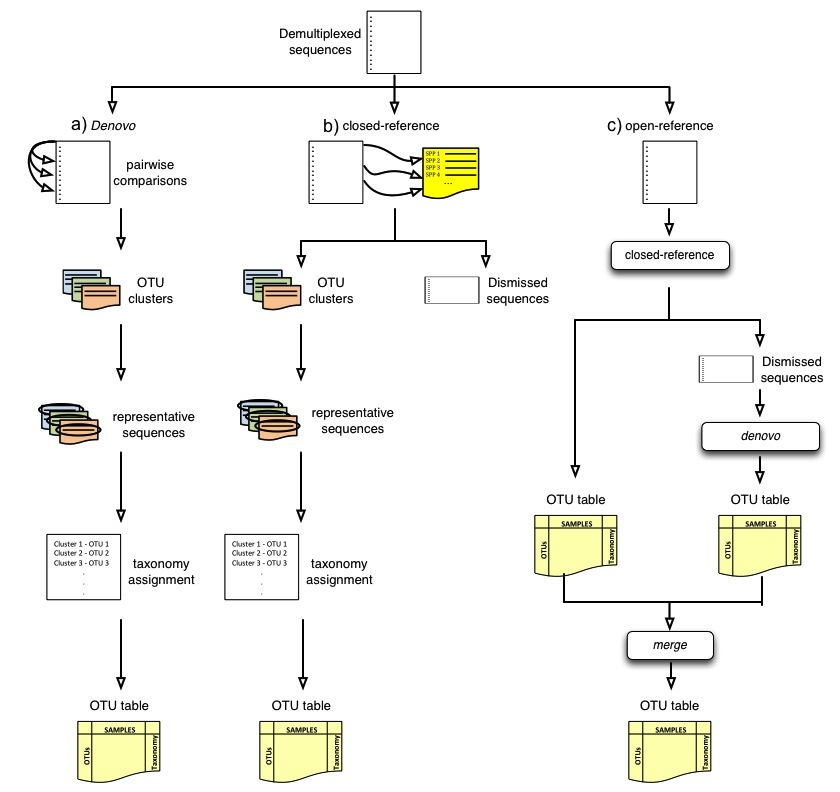
\includegraphics[width=0.75\columnwidth]{chapter_book_figures/Figure_2.jpg}
\caption[Cartoon representation of the \gls{otu} picking approaches]{\textbf{Cartoon representation of the \gls{otu} picking approaches.}
(a) de novo, (b) closed-reference and (c) open reference \gls{otu} picking respectively.
In the de novo method, sequences are compared to each other and then clusters are formed.
In the closed-reference method, sequences are compared directly to a reference dataset (e.g. GreenGenes).
Sequences that match a reference sequence are clustered; the remaining sequences are discarded. I
both \gls{otu} picking methods, once clusters are formed, a representative sequence is selected and
then taxonomy is assigned to that sequence (and applied to the rest of the sequences that make up the \gls{otu}).
Open-reference combines the closed-reference and open-reference methods. The first step is identical to
closed-reference, sequences discarded in the first step are clustered into \gls{otu}s by the de novo method,
and both \gls{otu} tables are merged into a single final \gls{otu} table. De novo and open-reference cluster all
the sequences, but closed-reference allows better comparisons between studies, especially those using
different primers, because all \gls{otu}s occur in a common reference space.}
\label{bfigure2}
\end{figure}

The \gls{otu} picking strategies shown in Figure ~\ref{bfigure2} are built on top of
algorithms for de novo clustering. Of the various algorithms available, the furthest-neighbor,
average-neighbor or nearest neighbor in mothur \cite{Schloss2005, Schloss2009} (also named
complete linkage, average linkage, and single linkage respectively) are the most widely used.
Furthest-neighbor requires that each sequence is closer than the distance threshold to
every other sequence already in the \gls{otu} (Figure ~\ref{bfigure3}). Average-neighbor requires
that the average pairwise distance of all sequences in the \gls{otu} is closer than the
distance threshold. Nearest-neighbor requires that each sequence is closer than the
distance threshold to any sequence already in the \gls{otu}. Because these three algorithms
are variants on hierarchical clustering, they require loading the distance matrix
(proportional to the square of the number of dereplicated sequences) into memory, and are
therefore challenging to apply to large datasets (e.g., larger than 105 sequences). The
\gls{otu}s yield by these three algorithms also change their memberships at different sequencing depths
(i.e. the number of sequences chosen for clustering), which can be a problem for estimates of total
\gls{otu} numbers \cite{Roesch2007}.

\begin{figure}[htbp]
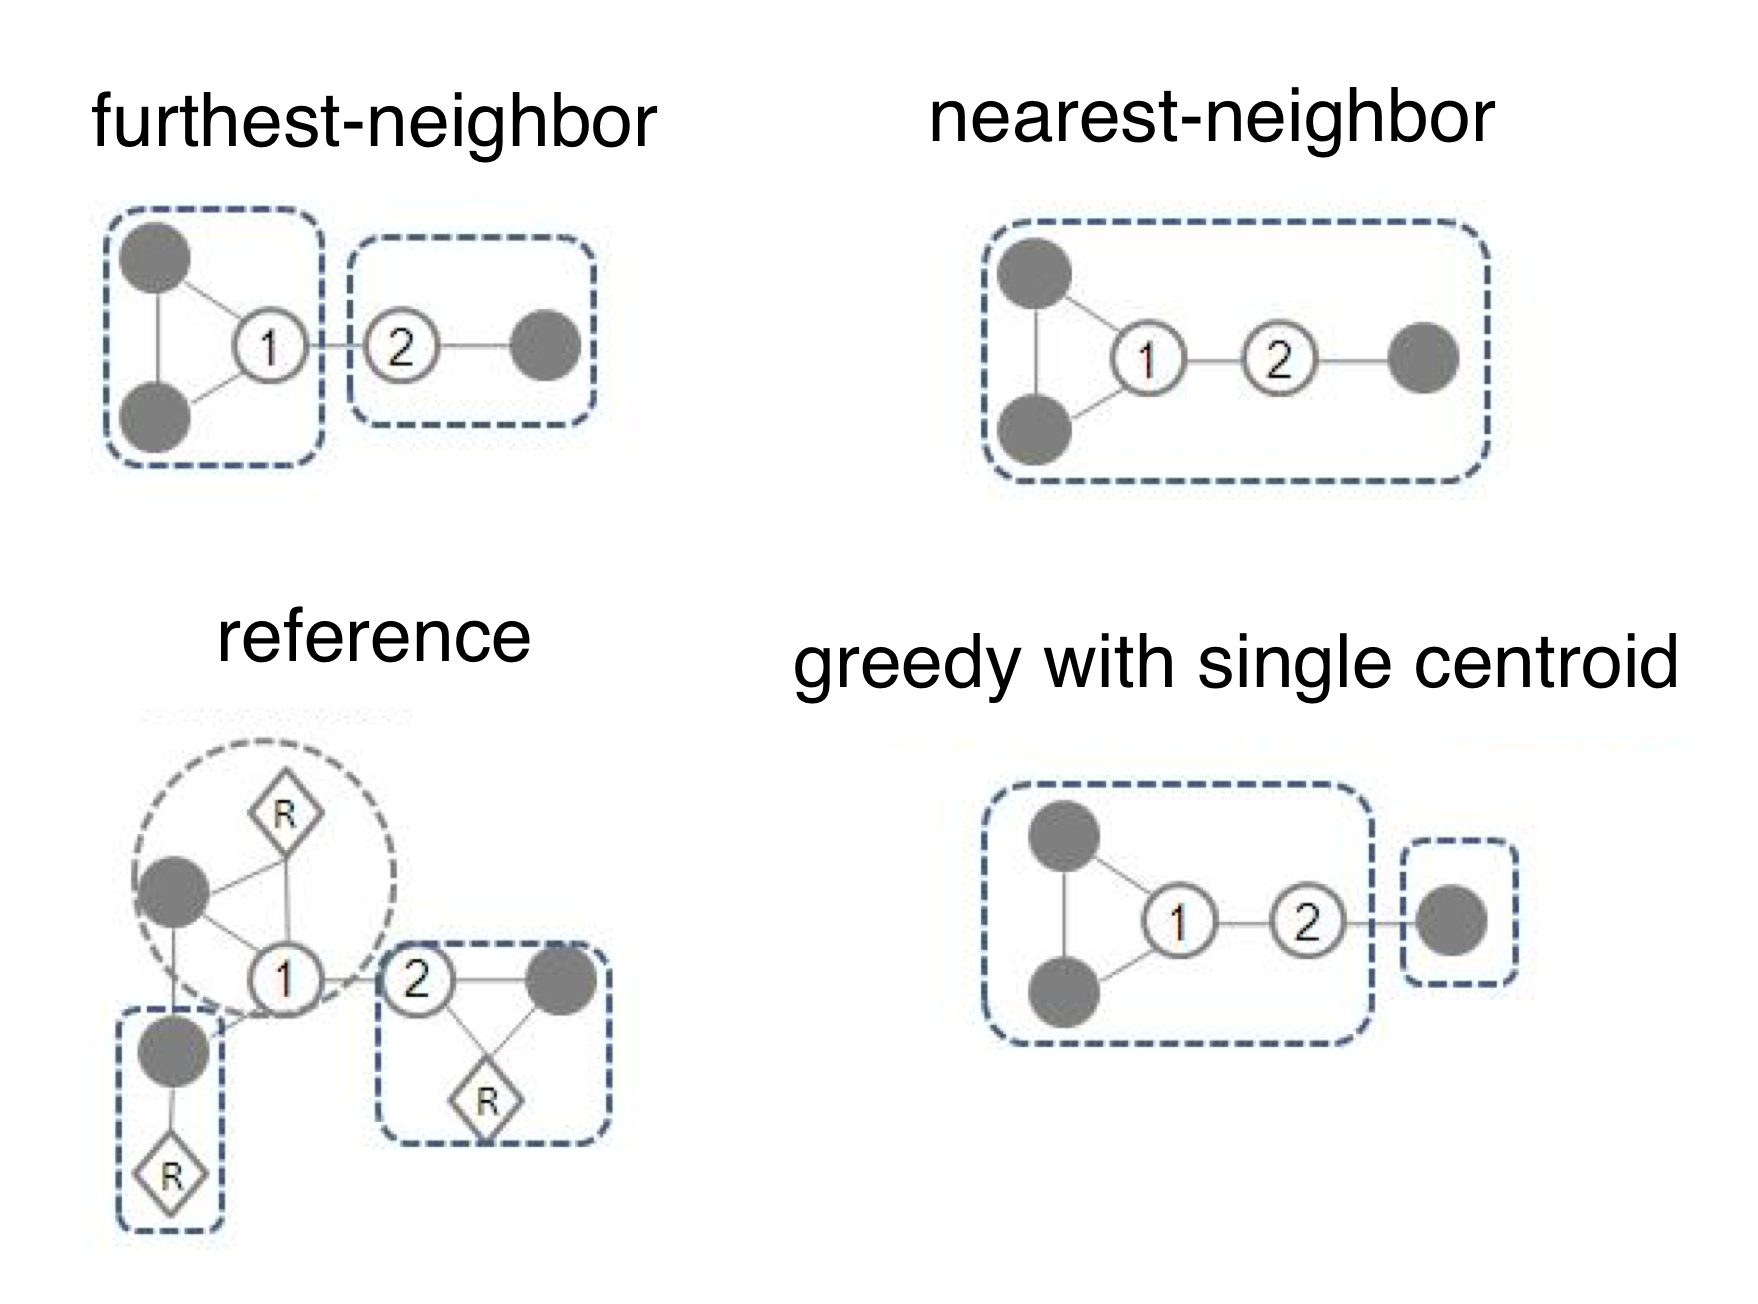
\includegraphics[width=0.75\columnwidth]{chapter_book_figures/Figure_3.jpg}
\caption[Cartoon demonstrating different clustering algorithms]{\textbf{Cartoon demonstrating different clustering algorithms.}
Circles representing sequences linked with lines are within the distance threshold.
The two numbered sequences are the first and second sequences in order in the file.
The reference algorithms only consider the distance between reference (R) and sequences.}
\label{bfigure3}
\end{figure}

A solution to the distance matrix problem comes from uclust and usearch, which are
greedy algorithms based on using a single centroid in each \gls{otu} \cite{Edgar2010}.
The centroid could be either from a reference database (usearch) or identified de
novo from the sequence dataset (both uclust and usearch) (Figure ~\ref{bfigure3}).
Sequences are serially compared to centroids in a user-defined order (usually decreasing
abundance). If a sequence falls within the distance threshold of more than one centroid,
the new sequence can either be grouped with the first centroid encountered, or the one
with the closest distance. Both uclust and usearch are much more efficient than the
hierarchical methods, and they do not need to load a large distance matrix into memory
(although recent versions of mothur also avoid the constraint of loading the full
distance matrix). usearch is the default de novo \gls{otu} picking method in \gls{qiime}.
Note that it is essential to note both your \gls{otu} picking strategy, and, if de novo
\gls{otu} picking is used, which algorithm you used to do it: it is not sufficient
simply to state that you used a 97\% threshold.

Because the \gls{otu} picking approach selection is a critical point in microbial
community analysis, the \gls{qiime} team has produced a detailed document that
describes the \gls{otu} picking protocols, their advantages and limitations
\footnote{\url{https://github.com/qiime/qiime/blob/master/doc/tutorials/otu_picking.rst}}.
Table ~\ref{btable3} compares the different \gls{otu} picking approaches and gives
guidelines for choosing an appropriate \gls{otu} picking strategy.

\begin{sidewaystable}[htbp]
\centering
\caption[\gls{otu} picking approaches comparison. The table shows when each of the \gls{otu} picking approaches should be used and when they cannot be applied. It briefly describes the advantages and disadvantages of using each of the \gls{otu} picking approaches.]{\gls{otu} picking approaches comparison. The table shows when each of the \gls{otu} picking approaches should be used and when they cannot be applied. It briefly describes the advantages and disadvantages of using each of the \gls{otu} picking approaches.}\label{btable3}
\renewcommand{\arraystretch}{0.5}% Tighter
\begin{tabular*}{\textwidth}{cccc}
& de novo & closed reference & open reference\\
\toprule
Must   & There is no reference          & Comparing non-overlapping. & -\\
use if & sequence collection to         & amplicons. The reference & \\
       & cluster against (e.g.          & set of sequences must span & \\
       & infrequently used              & both of the regions & \\
       & marker gene)                   & being sequenced & \\
\midrule
Cannot & Comparing non-overlapping   & There is no reference    & Comparing non-overlapping \\
use if & amplicons (e.g. V2 and      & sequence collection      & amplicons (e.g. V2 and V4\\
       &  V4 regions of 16S \gls{rrna})    & to cluster against       & regions of 16S \gls{rrna}). \\
       &                             & (e.g. infrequently       & There is no reference sequence\\
       &                             & used marker gene)        & collectionto cluster against \\
       &                             &                          & (e.g. infrequently used marker gene)\\
\midrule
Pros & All reads are clustered & Fast, as it is fully parallelizable    & All reads are clustered.\\
     &                         & (useful for extremely large datasets). & Fast, as is partially run on parallel.\\
     &                         & Better tree and taxonomy quality & \\
     &                         & since the \gls{otu}s are already defined & \\
     &                         & on the reference set. & \\
\midrule
Cons & Time consuming since it runs in         & Inability to detect novel      & There are still some steps\\
     & serial respect to the reference         & diversity with respect to      & performed in serial. If the\\
     & set because the reads that don’t        & the reference set because      & data set contains a lot of\\
     & hit the reference sequence collection   & the reads that don’t hit       & novel diversity with respect\\
     &  are discarded, so the analysis         & the reference sequence         & to the reference set, this\\
     & focus on the “already known” diversity. & collection are discarded,      & can still be slow.\\
     & If the studied environment is not       & so the analysis focus on       &\\
     & well-characterized, a large fraction    & the “already known” diversity. &\\
     & of the reads can be thrown away         & If the studied environment is  &\\
     &                                         & not well- characterized, a     &\\
     &                                         & large fraction of thereads     &\\
     &                                         & can be thrown away             &\\
\bottomrule
\end{tabular*}
\end{sidewaystable}
\renewcommand{\arraystretch}{1}% Restore original value

The recommended \gls{otu} picking approach is open-reference \gls{otu} picking,
because this approach provides the best trade-off between the time taken to complete
the analysis and the ability to discover novel diversity.

Once the sequences have been clustered into \gls{otu}s, a representative sequence
is picked for each \gls{otu}. The entire cluster will thus be represented by a single
sequence, speeding up subsequent steps (because redundant sequences need not be
considered). \gls{qiime} allows the representative sequence to be selected using
several techniques: choosing a sequence at random, choosing the longest sequence,
the most abundant sequence or the first sequence. If using uclust or usearch \cite{Edgar2010},
the cluster seed will be used as the representative sequence. The default behavior
in \gls{qiime} is to use the most abundant sequence in each \gls{otu} as the
representative sequence, because these sequences are least likely to represent
sequencing errors (for other applications, such as clustering with near-full-length
Sanger sequences, it may be more desirable to pick the longest sequence instead).
In case of closed-reference \gls{otu} picking, sequences from the reference collection
should be used as the representative sequences, which is the default behavior when
the closed-reference approach is selected.

\textbf{Identify chimeric sequences.} During the \gls{pcr} amplification process,
some of the amplified sequences can be produced from multiple parent sequences,
generating sequences known as chimeras. Although these sequences are technical
artifacts rather than representing actual members of the community, chimeric sequences
are important for alpha diversity estimates (although they are less important for
cross-sample comparisons, because each chimera is relatively rare and the same
chimera is unlikely to be generated systematically in different samples \cite{Ley2008}.
However, the same chimera can sometimes be generated in multiple \gls{pcr} reactions:
for example, Haas et al. \cite{Haas2011} reported that chimeric sequences formed
from Streptococcus and Staphylococcus occurred multiple times independently, so
presence of the same sequence in multiple \gls{pcr} does not mean that it is not chimeric.

\gls{qiime} currently supports three different methods for detecting chimeras: blast
fragments, a taxonomy-assignment-based approach using BLAST \cite{Altschul1990};
ChimeraSlayer \cite{Haas2011}, which uses BLAST to identify potential chimera parents;
and usearch 6.1 \cite{Edgar2010}, which can perform de novo chimera detection based on
abundances as well as reference-based chimera detection. The recommended method for
identifying chimeric sequences is uchime \cite{Edgar2011}, which is integrated in
the usearch 6.1 \cite{Edgar2010} pipeline. Uchime is the fastest method for detecting
chimeric sequences and it is executed by default if the usearch method is selected
for picking \gls{otu}.

\textbf{Taxonomy assignment.} The next step in the \gls{qiime} workflow is to
assign the taxonomy to each sequence of the representative set. This step connects
the \gls{otu}s to named organism, which is useful for inferring likely functional roles
for members of the community. When using a closed-reference approach for \gls{otu} picking,
the taxonomy of the sequences can be pulled out from the reference set. In case of
the open-reference and de novo approaches, because the clusters are not created from
any reference database (as a reminder, in the open-reference approach, sequences that
fail to cluster to the reference database form new clusters), the taxonomy should be
assigned using a reference dataset. We recommend the GreenGenes database
\cite{DeSantis2006, McDonald2012} as the default reference data set for assigning
taxonomy, although the RDP \cite{Cole2009} and Silva \cite{Quast2013} databases also
have strengths and weaknesses relative to GreenGenes and should be considered for some
analyses. Silva includes microbial eukaryotes and has invested substantial effort in
cleaning up marine taxa; RDP has close links to formally recognized names in taxonomy,
which can be especially useful for medical microbiology. \gls{qiime} can assign taxonomy
against any of the given databases, or against a custom database, using several
methods: BLAST \cite{Altschul1990}, RDP Classifier \cite{Wang2007}, rtax \cite{Soergel2012},
mothur \cite{Schloss2009} and tax2tree \cite{McDonald2012}. The \gls{qiime} team recommends
the RDP classifier method \cite{Wang2007} with a confidence value of 0.8. However, if
the user has paired-end reads, the best method to use is the rtax \cite{Soergel2012}, and
the user should provide the fasta files with both the first and second read from the
paired-end sequencing. Note that the taxonomy assignment method and the reference database
must both be described in order for an analysis to be reproducible, and that these methods
can have a larger effect on taxonomy than the underlying biological sample, so it is important
to be consistent \cite{Liu2008}.

\textbf{Sequence alignment.} The next step in the \gls{qiime} workflow is to align the
sequences. The sequences must be aligned to infer a phylogenetic tree, which is used for
diversity analyses and to understand the relationships among the sequences in the sample.
Currently, \gls{qiime} supports the following methods for performing sequence alignment:
PyNAST \cite{Caporaso2010PyNAST}, Infernal \cite{Nawrocki2009}, clustalw \cite{Larkin2007},
muscle \cite{Edgar2004} and mafft \cite{Katoh2002}. The recommended (and default) method is
PyNAST \cite{Caporaso2010PyNAST}. This method aligns the sequences against a template sequence
alignment, for which we recommend the GreenGenes core set \cite{DeSantis2006}.

When sequences do not align well using PyNAST, the Infernal package \cite{Nawrocki2009}
should be used. Like PyNAST, it requires a template alignment, but unlike PyNAST, it uses
\gls{scfg} to align incorporating secondary structure. Although this method is slow compared
to other methods, it does takes advantage of RNA secondary structure (provided in a
Stockholm-format file) and can be useful for aligning more variable \gls{rrna}s. For marker
genes other than \gls{rrna} genes, the best strategy for building phylogenetic trees is to align
the protein sequences (if available) using MUSCLE.

\textbf{Phylogeny construction.} This step in the \gls{qiime} workflow infers a
phylogenetic tree from the multiple sequence alignment generated by the previous step.
The phylogenetic tree represents the relationships among sequences in terms of the
amount of sequence evolution from a common ancestor. This phylogenetic tree is used
in many downstream analyses, such as the UniFrac metric \cite{Lozupone2005} for beta diversity.

The current methods supported for inferring the phylogenetic tree in \gls{qiime} are
FastTree \cite{Price2009}, clearcut \cite{Evans2006}, clustalw \cite{Larkin2007},
raxml \cite{Stamatakis2005} and muscle \cite{Edgar2004}. The default and recommended
method in \gls{qiime} is the FastTree \cite{Price2009} method because it shows the
best trade-off between run time and reliability of the inferred tree.

\textbf{Make \gls{otu} table} The last part of the upstream stage in \gls{qiime} is to
construct the \gls{otu} table. The \gls{otu} table is a sample by observation matrix
that also includes the taxonomic prediction for each \gls{otu}. For the \gls{otu} table
representation, \gls{qiime} uses the Genomics Standards Consortium candidate standard \gls{biom}
format \cite{McDonald2012BIOM}. The \gls{otu} table, the mapping file and the phylogenetic
tree, are the main files for performing the downstream analysis.

\gls{qiime} can perform all the steps for generating the \gls{otu} table and the
phylogenetic tree from the preprocessed data in a single command. There is a separate
command for each \gls{otu} picking approach. In the following commands, we assume that
the GreenGenes reference files \cite{DeSantis2006} are located in the current directory.
As a remainder, our seqs.fna has 12.687.021 sequences of length 150.9989 +/- 0.1715:

\begin{itemize}
    \item For de novo (run time ∼80 hours on 1 processor (not parallelizable)):
    \begin{lstlisting}[language=bash]
    pick_de_novo_otus.py -i $PWD/slout/seqs.fna \
      -o $PWD/denovo_otus
    \end{lstlisting}
    \item For closed-reference (run time ∼2 hours on 20 processors):
    \begin{lstlisting}[language=bash]
    pick_closed_reference_otus.py -i $PWD/slout/seqs.fna \
      -o $PWD/closed_ref_otus \
      -r $PWD/gg_12_10_otus/rep_set/97_otus.fasta \
      -t $PWD/gg_12_10_otus/taxonomy/97_otu_taxonomy.txt \
      -a -O 20
    \end{lstlisting}
    \item For open-reference (run time ∼27 hours on 20 processors):
    \begin{lstlisting}[language=bash]
    pick_open_reference_otus.py -o $PWD/open_ref_otus \
     -i $PWD/slout/seqs.fna \
     -r $PWD/gg_12_10_otus/rep_set/97_otus.fasta \
     -a -O 20
    \end{lstlisting}
\end{itemize}


Because the closed-reference and open-reference \gls{otu} picking approaches can
be run in parallel, we use the $-a$ and $-O$ 20 options in order to run them using
20 processors.

\subsubsection{Downstream analysis steps}

Once we have generated the \gls{otu} table and the phylogenetic tree, we can start the
downstream analysis. At this point, we strongly recommend performing a second level
of quality-filtering, based on \gls{otu} abundance. The recommended procedure is to
discard those \gls{otu}s with a number of sequences less than 0.005\% of the total
number of sequences (see Bokulich et al. \cite{Bokulich2013} for a detailed description
of the effect of this parameter in further downstream analyses). \gls{qiime} executes the
\gls{otu} abundance quality-filtering step through the script filter\_otus\_from\_otu\_table.py:

\begin{lstlisting}[language=bash]
filter_otus_from_otu_table.py \
 -i $PWD/open_ref_otus/otu_table_mc2_w_tax_no_pynast_failures.biom \
 -o $PWD/open_ref_otus/otu_table_filtered.biom \
 --min_count_fraction 0.00005
\end{lstlisting}

This step greatly reduces the problem of spurious \gls{otu}s, most of which are
present at very low abundance.

\gls{qiime} 1.7.0 allows a first-pass view of common diversity analyses using a single
command: core\_diversity\_analysis.py. One of the parameters required by this command
is the sampling depth, the number of sequences that should be included in each sample
for diversity analyses. This is required, because many of the commonly used diversity
metrics are very sensitive to the number of sequences obtained per sample, such that
samples that are similar in the number of sequences that were obtained appear similar
to one another. This is bad because the number of sequences per sample is typically
a methodological artifact, not reflective of biological reality. The sampling depth
defines the size of the random subset of sequences that will be selected for each
sample for all subsequent diversity analyses.

The optimal sampling depth is data-dependent. There is no universal way of choosing a
rarefaction level, although heuristics can be applied. For example, if most samples have
more than 10,000 sequences and the rest range from 500 to 50 sequences per sample,
it would be recommended to use 10,000 as the rarefaction level. Although many studies
show marked variation in sequence depth with only a few “bad” samples, it is not always
easy to choose the rarefaction level. We strongly recommend rarefying over 1000
sequences/sample for Illumina MiSeq, because samples below this level often suffer
from other quality issues as well.

The information needed to choose the rarefaction level can be obtained from the
script print\_biom\_table\_summary.py, which shows summary information on the
\gls{otu} table such as the number of sequences, the number of \gls{otu}s, the
number of samples and the number of counts per sample, among others:

\begin{lstlisting}[language=bash]
print_biom_table_summary.py \
 -i $PWD/open_ref_otus/otu_table_filtered.biom

Num samples: 90
Num observations: 783
Total count: 10637688.0
Table density (fraction of non-zero values): 0.4289
Table md5 (unzipped): eb0f1d7fbb50bc31695dade31db1e198
Counts/sample summary:
 Min: 1.0
 Max: 493427.0
 Median: 99111.0
 Mean: 118196.533333
 Std. dev.: 94277.5956531
 Sample Metadata Categories: None provided
 Observation Metadata Categories: taxonomy
Counts/sample detail:
 BLANK4.732555: 1.0
 BLANK5.732537: 1.0
 Joshua.Jose.WTAbd.732533: 1.0
 Nick.Krishna.TG.Fec.732513: 2.0
 TH.CVA.WT.Oral.732491: 2.0
 BLANK2.732552: 3.0
 BLANK3.732479: 5.0
 BLANK6.732470: 7.0
 Elizabeth.Chris.WT.Abd.732490: 10.0
 Uri.Jake.TGAbd.732468: 10.0
 TH.CVA.WT.Abd.732477: 13.0
 BLANK10.732524: 812.0
 Elizabeth.Chris.WT.Oral.732520: 7410.0
 Elizabeth.Chris.WT.Col.732481: 21746.0
Jordan.Lisette.TG.Ile.732463: 27149.0
 ...
 TH.CVA.WT.Fec.732553: 372327.0
 Wang.TG.Cec.732527: 396391.0
 TH.CVA.WT.Ile.732517: 493427.0
\end{lstlisting}

In the above output we can see the information contained in the \gls{otu} table resulting
from applying the open-reference \gls{otu} picking. Some of the relevant information contained
in this output is the total number of samples (90), the total number of \gls{otu}s (783),
the number of reads (10637688) and the number of \gls{otu}s per sample. Applying the above
heuristic, we could select a subsampling depth of 7410 sequences. However, because we have
run three different \gls{otu} picking approaches and we want to compare them, we must search
for the rarefaction level that best fits the three \gls{otu} tables. Below are the summarized
information for the de novo \gls{otu} table and the closed reference \gls{otu} table, respectively:

\begin{lstlisting}[language=bash]
print_biom_table_summary.py \
 -i $PWD/denovo_otus/otu_table_filtered.biom
Num samples: 93
Num observations: 600
Total count: 11122386.0
Table density (fraction of non-zero values): 0.4344
Table md5 (unzipped): b002dd85c93fd9d0571ff23b05d21dde
Counts/sample summary:
 Min: 0.0
 Max: 497234.0
 Median: 108322.0
 Mean: 119595.548387
 Std. dev.: 93487.3335598
 Sample Metadata Categories: None provided
 Observation Metadata Categories: taxonomy
Counts/sample detail:
 BLANK7.732497: 0.0
 BLANK8.732522: 0.0
 Jordan.Lisette.TG.Abd.732467: 0.0
 BLANK4.732555: 1.0
 BLANK5.732537: 1.0
 Joshua.Jose.WTAbd.732533: 1.0
 BLANK2.732552: 3.0
 Nick.Krishna.TG.Fec.732513: 3.0
 TH.CVA.WT.Oral.732491: 3.0
 BLANK3.732479: 5.0
 BLANK6.732470: 9.0
 Elizabeth.Chris.WT.Abd.732490: 10.0
 Uri.Jake.TGAbd.732468: 10.0
 TH.CVA.WT.Abd.732477: 13.0
 BLANK10.732524: 825.0
 Elizabeth.Chris.WT.Oral.732520: 7376.0
 Joey.Aaron.Kyle.WT.Abd.732541: 35655.0
 ...
 Wang.TG.Cec.732527: 394351.0
 TH.CVA.WT.Ile.732517: 497234.0

print_biom_table_summary.py \
 -i $PWD/closed_ref_otus/otu_table_filtered.biom
Num samples: 90
Num observations: 673
Total count: 9434459.0
Table density (fraction of non-zero values): 0.4250
Table md5 (unzipped): 257b528478a2700c72f979ce8d9a9a1c
Counts/sample summary:
 Min: 1.0
 Max: 347785.0
 Median: 90092.0
 Mean: 104827.322222
 Std. dev.: 78560.4683831
 Sample Metadata Categories: None provided
 Observation Metadata Categories: taxonomy
Counts/sample detail:
 BLANK4.732555: 1.0
 BLANK5.732537: 1.0
 Joshua.Jose.WTAbd.732533: 1.0
 BLANK3.732479: 2.0
 Nick.Krishna.TG.Fec.732513: 2.0
 TH.CVA.WT.Oral.732491: 2.0
 BLANK2.732552: 3.0
 Uri.Jake.TGAbd.732468: 5.0
 BLANK6.732470: 7.0
 Elizabeth.Chris.WT.Abd.732490: 10.0
 TH.CVA.WT.Abd.732477: 12.0
 BLANK10.732524: 710.0
 Elizabeth.Chris.WT.Oral.732520: 7205.0
 Elizabeth.Chris.WT.Col.732481: 22652.0
 ...
 TH.CVA.WT.Fec.732553: 329988.0
 TH.CVA.WT.Ile.732517: 347785.0
\end{lstlisting}

From the above output, we see that a reasonable rarefaction level for the three
tables is 7205 counts per sample, derived from the closed reference \gls{otu} picking.

Once the subsampling depth is chosen, we can execute the core\_diversity\_analyses.py
command over the three \gls{otu} tables. We provide the subsampling depth via the
$-e$ parameter, the \gls{otu} table via the $-i$ parameter, the mapping file through
the $-m$ parameter and the metadata categories to use in categorical analyses through
the $-c$ parameter. The $-o$ parameter is used to provide the output directory and the
$-a -O$ 64 are used to run the command in parallel using 64 processes.

\begin{lstlisting}[language=bash]
mkdir $PWD/diversity_analysis

core_diversity_analyses.py \
 -i $PWD/open_ref_otus/otu_table_filtered.biom \
 -m $PWD/IQ_Bio_16sV4_L001_map.txt \
 -t $PWD/open_ref_otus/rep_set.tre \
 -e 7205 -c GENOTYPE,BODY_SITE \
 -o $PWD/diversity_analysis/open_ref -a -O 64

core_diversity_analyses.py \
 -i $PWD/denovo_otus/otu_table_filtered.biom \
 -m $PWD/IQ_Bio_16sV4_L001_map.txt \
 -t $PWD/denovo_otus/rep_set.tre -e 7205 \
 -c GENOTYPE,BODY_SITE \
 -o $PWD/diversity_analysis/denovo -a -O 64

core_diversity_analyses.py \
 -i $PWD/closed_ref_otus/otu_table_filtered.biom \
 -m $PWD/IQ_Bio_16sV4_L001_map.txt \
 -t $PWD/gg_12_10_otus/trees/97_otus.tree \
 -e 7205 -c GENOTYPE,BODY_SITE \
 -o $PWD/diversity_analysis/closed_ref -a -O 64
\end{lstlisting}

The core\_diversity\_analyses.py command filters the \gls{otu} table before
executing the diversity analyses. The filter removes samples from the \gls{otu}
table that do not have at least the user-defined subsampling depth (7205 in our
case). This filtering removes low-coverage samples from the \gls{otu} table, because
they are not informative enough to be included in the study. After these samples
have been filtered, the script performs the rarefaction step at the given subsampling depth.

The output of this script is an HTML file that can be opened in a web browser (Figure ~\ref{bfigure4}).
This HTML file gives access to the results of the different diversity analysis performed
(taxa summaries, $\alpha$-diversity, $\beta$-diversity and category significance)
which will be explained in further sections.

\begin{figure}[htbp]
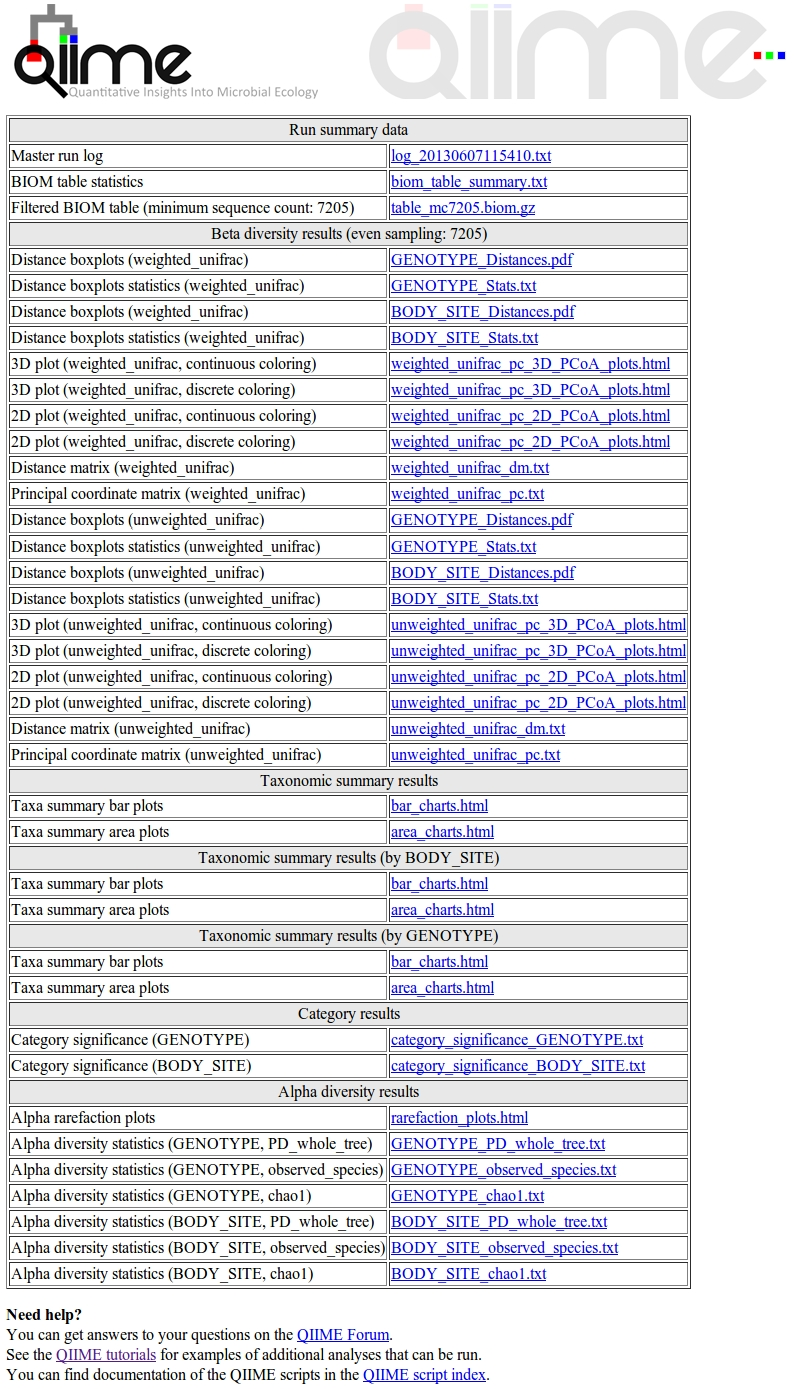
\includegraphics[width=0.75\columnwidth]{chapter_book_figures/Figure_4.jpg}
\caption[HTML result from core\_diversity\_analyses.py]{\textbf{HTML result from core\_diversity\_analyses.py.}
This HTML file summarizes and gives access to the results of the diversity analyses conducted on the given \gls{otu} table}
\label{bfigure4}
\end{figure}

For the following downstream analysis we have used the \gls{otu} table and phylogenetic
tree resulting from the open-reference \gls{otu} picking approach. In cases where we
are performing comparisons between \gls{otu} picking approaches, we will specify
which approaches we have used.

\textbf{Taxa summaries.} One way to visualize the \gls{otu}s in each sample is a taxa
summary, which summarizes the relative abundance of the taxa present in a set of
samples on multiple taxonomic levels (e.g. phylum, order, etc.) (see Figure ~\ref{bfigure5}).
This provides a quick way to identify samples that may be drastically different from others
(i.e. outliers), and visually identify expected patterns and differences between and among samples.
For example, this tool can be used to identify patterns such as differences in the
relative abundance of Firmicutes and Bacteroidetes in the gut microbiomes of lean versus
obese mice, e.g. Ley, Backhed, Turnbaugh, Lozupone, Knight, and Gordon \cite{Ley2008}.
These patterns can then be statistically tested using other methods, either within \gls{qiime} or
elsewhere. \gls{qiime} contains a workflow called summarize\_taxa\_through\_plots.py that generates
user-specified plot types, including bar, pie, and area graphs. These graphs provide a way to
visually compare the composition of each sample, or of groups of samples. An \gls{otu} table
with assigned taxonomies is the only required input file, and options allow the user
summarize across categories (using the metadata file), at different taxonomic levels, or
only using \gls{otu}s that are present at abundances higher or lower than user-defined thresholds.
The web interface allows a scroll-over feature that identifies the taxonomy of the separate taxa.
Additional output files include image files of the charts and legends, and tab-delimited files
of the calculated abundances, which can then be further filtered and manipulated for
downstream statistical analyses.

\begin{figure}[htbp]
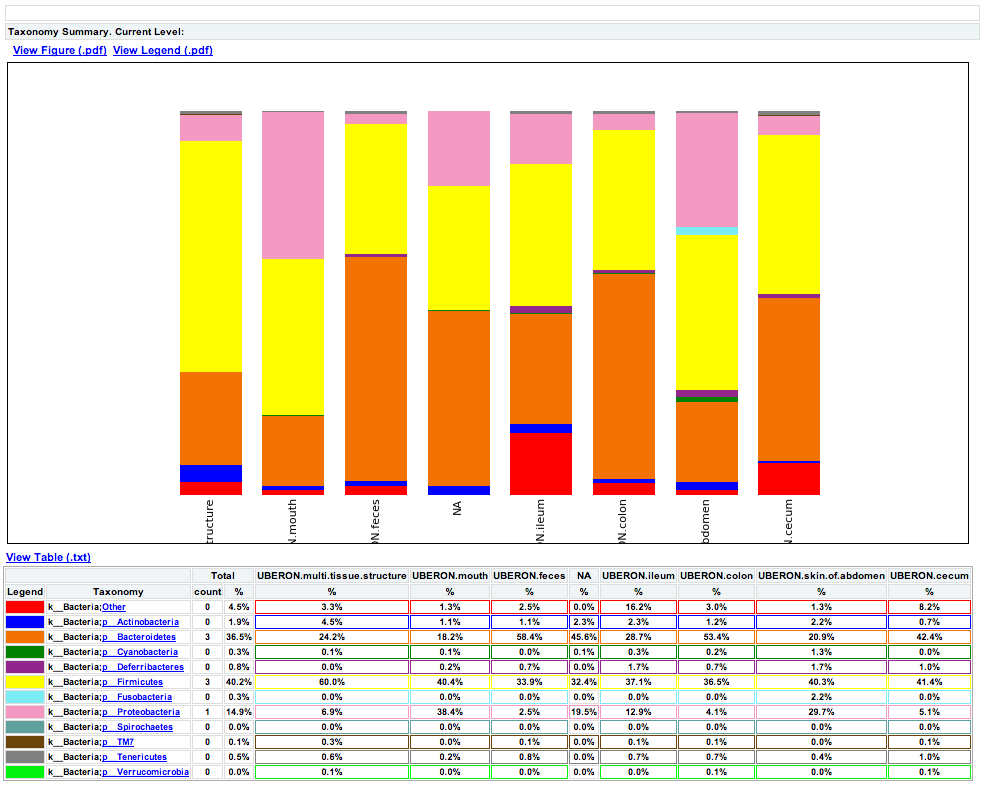
\includegraphics[width=0.75\columnwidth]{chapter_book_figures/Figure_5.jpg}
\caption[Taxa summary of the example dataset]{\textbf{Taxa summary of the example dataset.}
Samples have been grouped and averaged by body site, and taxonomic composition is shown on
the phylum level. Each column in the plot represents a body site, and each color in the column
represents the percentage of the total sample contributed by each taxon group at phylum level.
The taxa summaries plot help us to see which taxon groups are more prevalent in a sample.
For example, the fecal samples are dominated by Bacteroidetes, while mouth and skin samples
are dominated by Proteobacteria. We can also see that Fusobacteria is only present at appreciable
levels in the skin samples.}
\label{bfigure5}
\end{figure}

\textbf{Diversity analysis.} Microbial ecology studies the diversity of microorganisms
by characterizing bacterial communities in different environments, and determining the
factors that drive diversity in these communities \cite{Atlas1998}. Whittaker (1960) and
Whittaker (1972) define different types of measurements of diversity as alpha, beta and gamma
diversities. Alpha diversity is defined as the diversity of organisms in one sample or environment.
Beta-diversity is the difference in diversities across samples or environments. Finally,
gamma-diversity ($\gamma$-diversity) measures the diversity at a broader scale, such as a
province or region. Several different metrics of alpha- and beta-diversity are implemented in in
\gls{qiime} pipeline. Diversity measurements and their applications in microbial have been discussed in
detail elsewhere \cite{Jost2007, Kuczynski2010Patterns, Lozupone2008}, and here we focus on
examples of their application.

\textbf{Alpha diversity analysis.} \gls{qiime} can generate plots showing the results of
alpha diversity, allowing the user to choose the diversity metric and different
rarefaction levels (Figure ~\ref{bfigure6}). These images are often used to estimate
the true species richness of a community.

\begin{figure}[htbp]
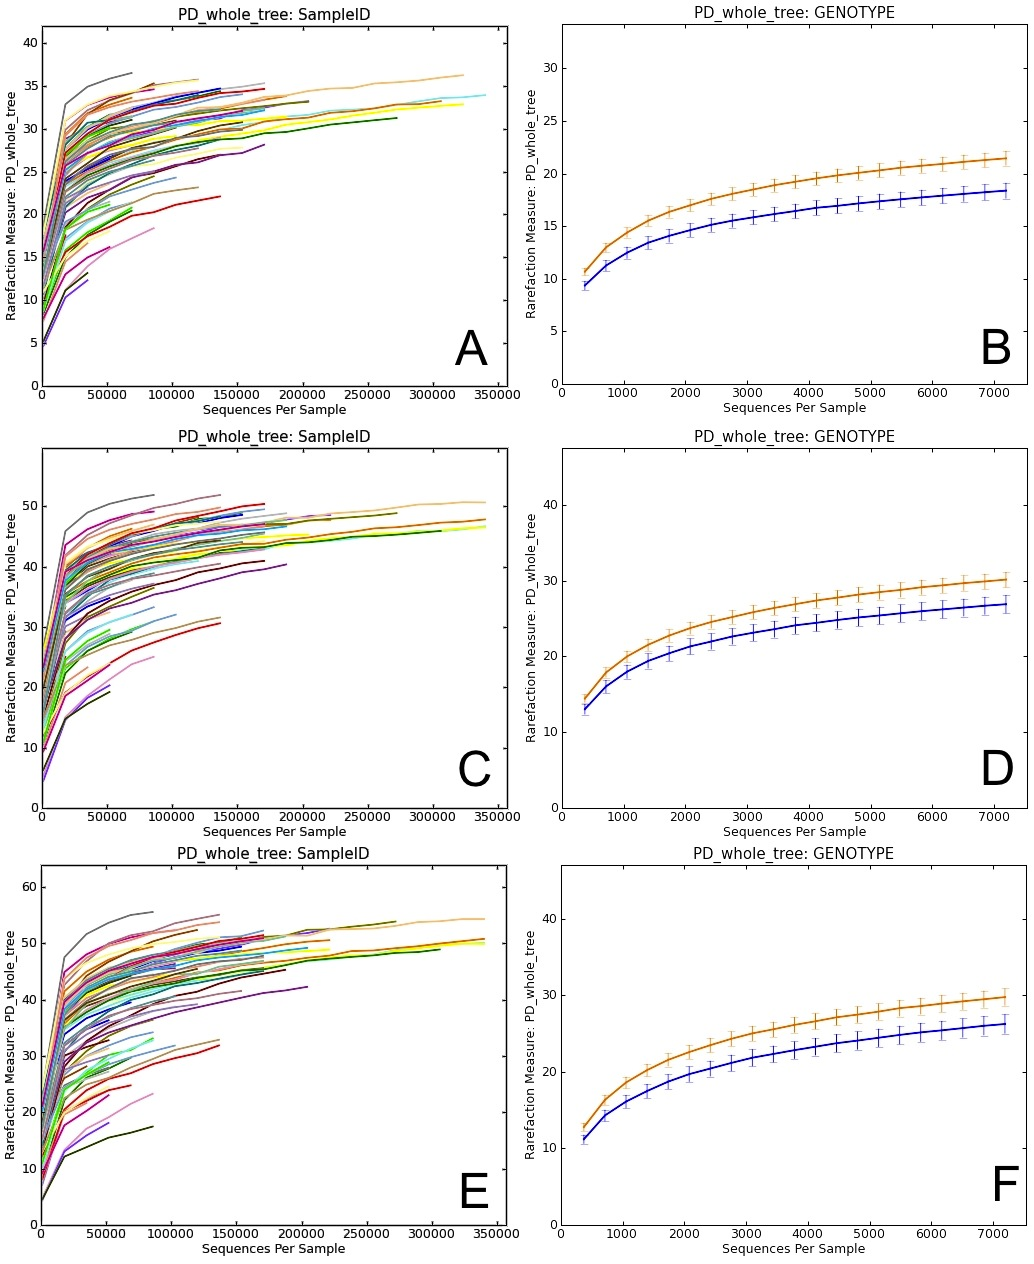
\includegraphics[width=0.75\columnwidth]{chapter_book_figures/Figure_6.jpg}
\caption[Alpha diversity curves at different rarefaction depths using different \gls{otu} picking methods]{\textbf{Alpha diversity curves at different rarefaction depths using different \gls{otu} picking methods.}
Each line represents the results of the alpha diversity phylogenetic diversity whole
tree metric (PD Whole Tree in \gls{qiime}). A, C and E represent alpha diversity of each sample
at a different sequence depth in each of the \gls{otu} picking protocols (closed-, open-reference and
de novo). In closed-reference, the diversity plateaus (reaches an asymptote) because only \gls{otu}s
in the reference database already can be considered, greatly reducing the \gls{otu} number over what
is possible if the sequences are clustered de novo. Comparing these curves is difficult because
the sequencing depth differs among samples. B, D and F show differences in alpha diversity between
the two mouse genotypes, wild type (WT - orange) and transgenic (TG - blue), using the different
\gls{otu} picking approaches. Both curves show the same rarefaction levels, allowing easier comparisons
between categories. The curves again level off, showing that the sequencing effort is sufficient
to detect most of the \gls{otu}s (this saturation can be confirmed using Good's coverage, or conditional
uncovered probability, or other formal coverage statistics). The error bars show the standard error
of the mean diversity at each rarefaction level across the multiple iterations.}
\label{bfigure6}
\end{figure}

\gls{qiime} implements dozens of the most widely used alpha diversity indices, including both
phylogenetic indices (which require a phylogenetic tree) and non-phylogenetic indices. Users
can obtain a list of the alpha diversity indices implemented in \gls{qiime} by passing the parameter
$–s$ to the alpha\_diversity.py script. Phylogenetic metrics have been especially useful
in our experience because they provide additional power by accounting for the degrees of
phylogenetic divergence between sequences within each sample. Thus, for alpha diversity,
we recommend Phylogenetic Distance (PD) \cite{Faith1992} over \gls{otu} counts; however, the choice
of metric will depend on the question. In particular, one might be interested in pure
estimates of community richness (such as the observed number of \gls{otu}s, or the Chao1 estimator
of the total number that would be observed with infinite sampling), in pure estimates of
evenness, or of measures that combine richness and evenness such as the Shannon entropy
(if there is no hypothesis in advance about which richness measure is appropriate, remember
to correct for multiple comparisons if many are applied to the same dataset). Here is an example
of how to compute rarefaction curves for three different alpha diversity metrics using a \gls{qiime} parameters file:

\begin{lstlisting}[language=bash]
echo “alpha_diversity:metrics shannon,PD_whole_tree,observed_species” \
 > alpha_params.txt

alpha_rarefaction.py \
 -i $PWD/open_ref_otus/otu_table_filtered.biom \
 -m $PWD/IQ_Bio_16sV4_L001_map.txt \
 -o $PWD/diversity_analysis/alpha_rare_open_ref_uneven \
 -a -O 64 -n 20 --min_rare_depth 1000 -e 340000 \
 -p $PWD/alpha_params.txt \
 -t $PWD/open_ref_otus/rep_set.tre
\end{lstlisting}

This step generates an interactive HTML document with figures showing the
results for each alpha diversity metric and for each group of samples. Curves
reach asymptotes when the sequencing effort (sequencing depth) does not contribute
additional \gls{otu}s. In this sense, curves would differ in their shape as a function
of the selected \gls{otu} picking method.

Comparisons should be adjusted to the same depth of sequencing. Rarefaction curves
can be useful for assessing the sequencing effort sufficient for representing and
comparing the microbial communities (Figure ~\ref{bfigure6}). However, although
rarefaction curves were widely used during the era of Sanger sequencing, when most
communities were undersampled, it is often more useful today to report the coverage
and the estimated and observed numbers of \gls{otu}s at one rarefaction depth rather than
to use a figure for rarefaction curves.

\textbf{Beta diversity analysis.} Beta diversity can also be calculated from the rarefied \gls{otu} tables, comparing the
microbial communities based on their compositional structures. As with alpha diversity,
\gls{qiime} can compute many phylogenetic and non-phylogenetic beta diversity metrics (shown
by the command beta\_diversity.py $-s$).Of these, we have found UniFrac to be most
generally useful in revealing biologically meaningful patterns. Unifrac measures
the amount of unique evolution within each community with respect to another by
calculating the fraction of branch length of the phylogenetic tree that is unique
to either one of a pair of communities \cite{Lozupone2005}. \gls{qiime} implements several
variants of Unifrac, including weighted and unweighted Unifrac. The weighted Unifrac
metric is weighted by the difference in probability mass of \gls{otu}s from each community
for each branch, whereas unweighted Unifrac only consider the absence/presence of the
\gls{otu}s \cite{Lozupone2007}. Weighted Unifrac is thus recommended for detecting community
differences that arise from differences in relative abundance of taxa, rather than in
which taxa are present. Like other metrics considering taxon abundance, weighted Unifrac
is sensitive to the bias from DNA extraction efficiency, PCR amplification, etc.; this may
explain why, in our hands at least, unweighted UniFrac has often provided results that
correlate better with clinical or environmental variables than does weighted UniFrac.
The choice of metrics is critical in beta diversity analysis as metrics differ substantially
in their ability to detect clustering or gradient patterns among microbial communities on
the same dataset \cite{Arumugam2011, Ravel2012, Schloss2006}. See
Kuczynski et al. \cite{Kuczynski2010Patterns} for a detailed discussion of the performance
of different nonphylogenetic metrics.

\gls{qiime} calculates the beta diversities between each pairs of input samples, forming a
distance matrix. The distance matrix then can be visualized with methods such as \gls{pcoa}
and hierarchical clustering, both of which have been widely used for data visualization
for decades. \gls{pcoa} transforms the original multidimensional matrix to a new set of
orthogonal axes that explain the maximum amount of inertia in the dataset and the
current implementation in \gls{qiime} scales to thousands of samples. We are currently
evaluating approximate methods that will allow scaling to millions of samples \cite{Gonzalez2012}.
\gls{qiime} allows the \gls{pcoa} plots to be visualized interactively in 3-dimensions,
currently using the KiNG viewer \cite{Chen2009}. To assess the stability of the \gls{pcoa} plot,
jackknife resampling can be performed on the \gls{otu} table, repeating the \gls{pcoa} procedure for
each resampled table and plotting the aggregate results as confidence ellipsoids around
the sample points (Figure ~\ref{bfigure7}). Jackknifing is recommended because many diversity
metrics, including UniFrac, are sensitive to the number of sequences per sample \cite{Lozupone2011}.

\begin{figure}[htbp]
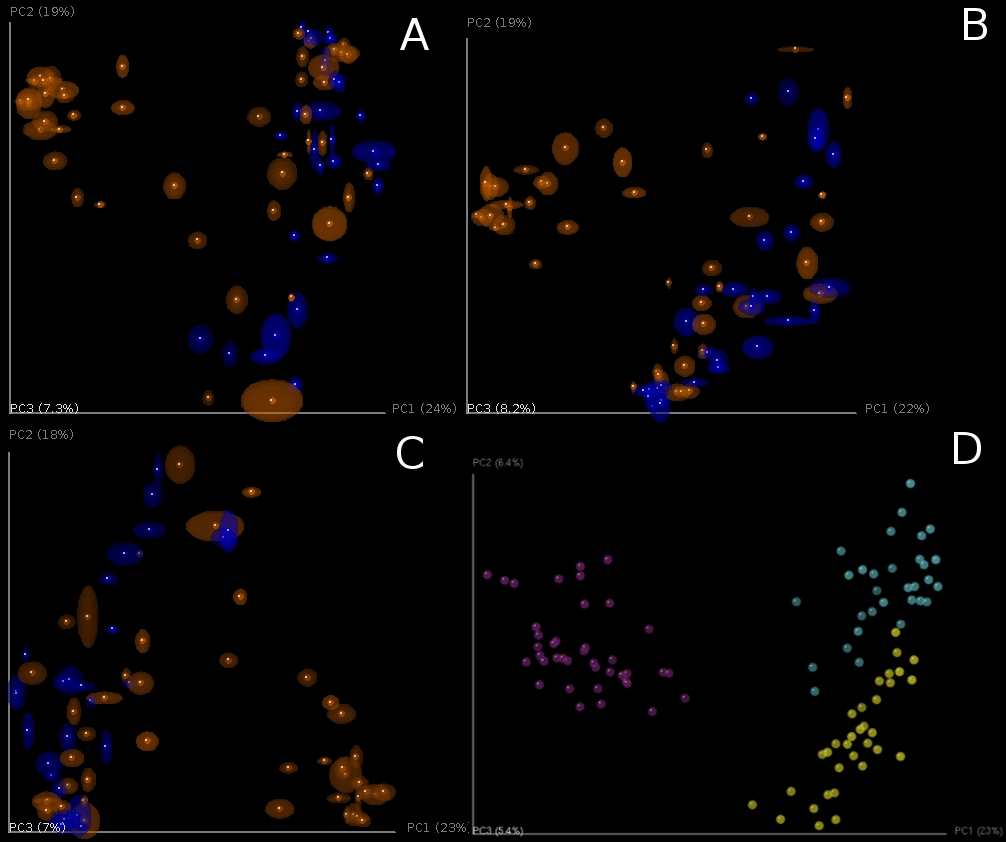
\includegraphics[width=0.75\columnwidth]{chapter_book_figures/Figure_7.jpg}
\caption[PCoA plots of unweighted Unifrac beta diversity]{\textbf{PCoA plots of unweighted Unifrac beta diversity.}
Panels A-C shows jackknifed replicate results for the example data set using de novo \gls{otu} picking,
closed-reference \gls{otu} picking and open-reference \gls{otu} picking, illustrating different results from the
three \gls{otu} picking approaches (Table ~\ref{btable3}). Each dot represents a sample, either from a WT
mouse (orange) or TG mouse (blue). The two groups are not clearly separated, probably because the
data set is contaminated (recall that this is a class project and different participants varied in
their dissection skills). The size of the ellipsoids show the variation for each sample calculated
from jackknife analysis. These plots are generated by the command jackknifed\_beta\_diversity.py
-i \$PWD/denovo\_otus/otu\_table\_filtered.biom -t \$PWD/denovo\_otus/rep\_set.tre -m \$PWD/IQ\_Bio\_16sV4\_L001\_map.txt
-o \$PWD/diversity\_analysis/jk\_denovo -e 7205 -a -O 64 (the input parameters should be adapted for using
the \gls{otu} tables from different \gls{otu} picking approaches). Panel D shows the beta diversity PCoA plot of a data set
from the “keyboard” data set \cite{Fierer2010} which links individuals to their computer keyboard through
microbial community similarity. Each dot represents a microbial community sampled from either fingertips or
keyboard keys from three individuals, annotated by the three colors shown in the plot. In contrast to panels A-C,
Panel D shows the microbial communities well-separated by individual in the PCoA plot.}
\label{bfigure7}
\end{figure}

Taxonomic information can be displayed on top of the PCoA using biplots (Figure ~\ref{bfigure8})
(this analysis requires the output file from previous taxon summary step). The coordinates
of a given taxon are computed as the weighted average of the coordinates of all samples,
where the weights are the relative abundances of the given taxon in the set of samples.
This plot is particularly suited for identifying taxa that drive the differentiation
between groups of microbial communities.

\begin{figure}[htbp]
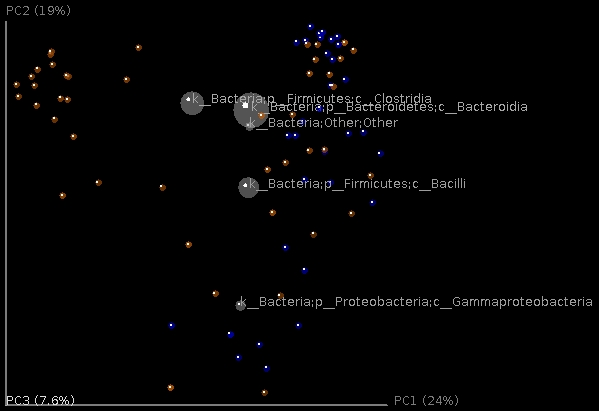
\includegraphics[width=0.75\columnwidth]{chapter_book_figures/Figure_8.jpg}
\caption[Biplot of the example data set]{\textbf{Biplot of the example data set.}
This is the unweighted Unifrac beta diversity plot, similar to Figure ~\ref{bfigure7},
with labels for the most 5 abundant phylum-level taxa added. The size of the sphere
for each taxon is proportional to the mean relative abundance of that taxon across all
samples. This plot is created by the command make\_3d\_plots.py -i
\$PWD/diversity\_analysis/open\_ref/bdiv\_even7205/unweighted\_unifrac\_pc.txt -m
\$PWD/IQ\_Bio\_16sV4\_L001\_map.txt -t
\$PWD/diversity\_analysis/open\_ref/taxa\_plots/table\_mc7205\_sorted\_L3.txt
--n\_taxa\_keep 5 -o \$PWD/diversity\_analysis/3d\_biplot}
\label{bfigure8}
\end{figure}

Another popular method for finding relationships among samples is hierarchical clustering,
which groups samples together into a tree. Although hierarchical clustering can be effective
in some cases, it should be used with caution because the eye can easily be drawn to incorrect
relationships (such as samples that are adjacent in terms of the order of their labels but are topologically
far apart in the tree). In general, we recommend using PCoA as a method of detecting grouping in the data,
but demonstrate hierarchical clustering here as an example. Here we analyze the beta diversity
distance matrix using UPGMA, which forces the samples into an ultrametric tree (i.e. a tree in
which the distance from the roots to the tips is the same for every tip) (Figure ~\ref{bfigure9}).
The resulting tree file is in Newick format, and can be visualized by programs including
TopiaryExplorer \cite{Pirrung2011}, the R package ape \cite{Paradis2004} and the package
distory \cite{Chakerian2012}. UPGMA can also be applied to the jackknifed subsamples to
provide an estimate of the statistical confidence in the clustering, by showing the
frequency of each nodes in the original full data set cluster that are supported by the
jackknife replicates. We generally recommend against the use of hierarchical clustering
as a method for identifying and visualizing sample groupings, so have not invested as
much effort in enabling this technique in \gls{qiime} as has been invested in other
visualizations. However, if you do plan to use hierarchical clustering, it is important
to be aware that substantial work has been done on more effective visualization
methods, e.g. in distory \cite{Chakerian2012}, and performing additional analyses
outside \gls{qiime} may allow improvements over the default visualizations.

\begin{figure}[htbp]
\includegraphics[width=0.75\columnwidth]{chapter_book_figures/Figure_9.jpg}
\caption[Bootstrapped UPGMA clustering on the example data set]{\textbf{Bootstrapped UPGMA clustering on the example data set.}
The tree is shown with the internal nodes colored by bootstrap support (red: 75-100\%,
yellow: 50-75\%, green: 25-50\% and blue: $<$ 25\%). Although this visualization
is popular in the literature, we generally recommend alternatives such as PCoA.}
\label{bfigure9}
\end{figure}

\textbf{Statistical significance of differences in alpha and beta diversity.} Which
statistical tests should be applied depends on the particular hypotheses and predictions
defined \emph{a priori} in a given research study. \gls{qiime} implements several scripts
that perform a broad range of statistical tests between samples or groups of samples
using both alpha and beta diversity measurements. For alpha diversity, the
compare\_alpha\_diversity.py script performs comparisons between groups of samples.
The script uses the alpha diversity measurements of samples standardized to a given number
of sequences per sample, and performs nonparametric two-sample t-tests (i.e. using Monte Carlo
permutations to calculate the p-value) comparing each pair of groups of samples.
Rarefaction is a critical step in these analyses, as noted above, because typically diversity
estimates depend on the number of sequences per sample. At the maximum rarefaction depth,
wild type and transgenic mice did not show differences in alpha diversity as measured by PD
metric (wild type: (mean +/- sd) = 45.19 +/- 10.6; transgenic: 40.01 +/- 9.5; t = -2.17, p = 0.102).
We also tested for differences in alpha diversity between body sites. We found differences
between cecum and ileum (cecum (mean +/- s.d.) = 51.1 +/- 3.6; ileum: 36.72 +/- 8.2; t = 5.35, p = 0.028),
cecum and mouth (mouth: 29.54 +/- 10.1; t = 6.62, p = 0.028) and feces and
mouth (feces: 48.4 +/- 4.0; t = 5.47, p = 0.028). None of the other pairs of comparisons
between body sites showed significant differences in alpha diversity (colon: 46.0 +/- 9.2;
multi-tissue: 46.26 +/- 9.1; skin: 42.13+/- 7.4; all p-values $>$ 0.056).

The appropriate statistical tests of beta diversity also depend on the research question
being asked. These tests compare sets of distances between samples in the distance matrix.
Careful attention must be paid both to Type I error (rejecting the null hypothesis when it is actually
true), and to Type II error (accepting the null hypothesis when it is actually false, i.e. lack of
statistical power). Type I error is more likely when variance is unequal between groups, and when
many comparisons are performed on the same data (although multiple comparisons corrections correct
for the increased Type I error, they often raise the Type II error rate instead). As always,
results should be interpreted with caution and common sense. A highly statistically significant
result stemming from data with a low correlation coefficient may indicate that a relationship
has little biological meaning, and examining the scatterplot to see if the result is driven by a
few outliers would be prudent. Further theoretical validation (especially of the multivariate
statistical tests) is also needed, especially because the distributions underlying microbial
community data have in general not yet been well characterized.

Comparisons between distance matrices are performed in \gls{qiime} using the
compare\_distance\_matrices.py script. This script can perform analyses including
the Mantel test, the Partial Mantel test, and the Mantel Correlogram. The Mantel
test is a non-parametric test that compares two distance matrices, and calculates
a correlation coefficient and a significant p-value using permutations that preserve
the rows and columns. For the purpose of showing some examples (because the mouse
data does not include a time series component), we will use the sequence dataset published
by Caporaso et al. \cite{Caporaso2011}, where the authors studied variation in the
bacterial community in the human gut over time series. We will compare the Unifrac
distance matrix and a distance matrix as differences in days since the treatment started.
Both distance matrices showed a significant correlation (Mantel test: p = 0.035),
showing that bacterial communities were more similar as they were close in sampling.
The Mantel test measures the overall correlation between distance matrices, but Mantel Correlograms
measure this effect when taking into account the distances between samples marked by specific
metadata variables. Essentially, the second distance matrix (in our case, days since the
treatment started) is divided into classes. The classes into which the second distance
matrix (days after experiment started) is determined by Sturge's rule, a method for
determining the width of bars in a histogram based on the binomial formula. Then Mantel
tests are run between these distance classes and the beta diversity distance matrix.
We found that none of the distance classes were significantly related to the bacterial
community (Figure ~\ref{bfigure10}: all comparisons p $>$ 0.120, after Bonferroni correction
for multiple comparisons). The Mantel test showed us that there is an overall correlation between
bacterial community and “days after the experiment started” (samples collected closer in
time had more similar bacterial communities), and Mantel Correlogram showed that there is
no significant correlation between the bacterial community and any of the classes into which
the “days after the experiment started” matrix was divided. In other words, in this
case, discretization of the data into a few timepoint classes led to an undetectable pattern;
in contrast, use of the whole time series yielded an interpretable result. However, in other
datasets, the reverse is often true, especially if the variation is not monotonic
(e.g. in the case of seasonal variation).

\begin{figure}[htbp]
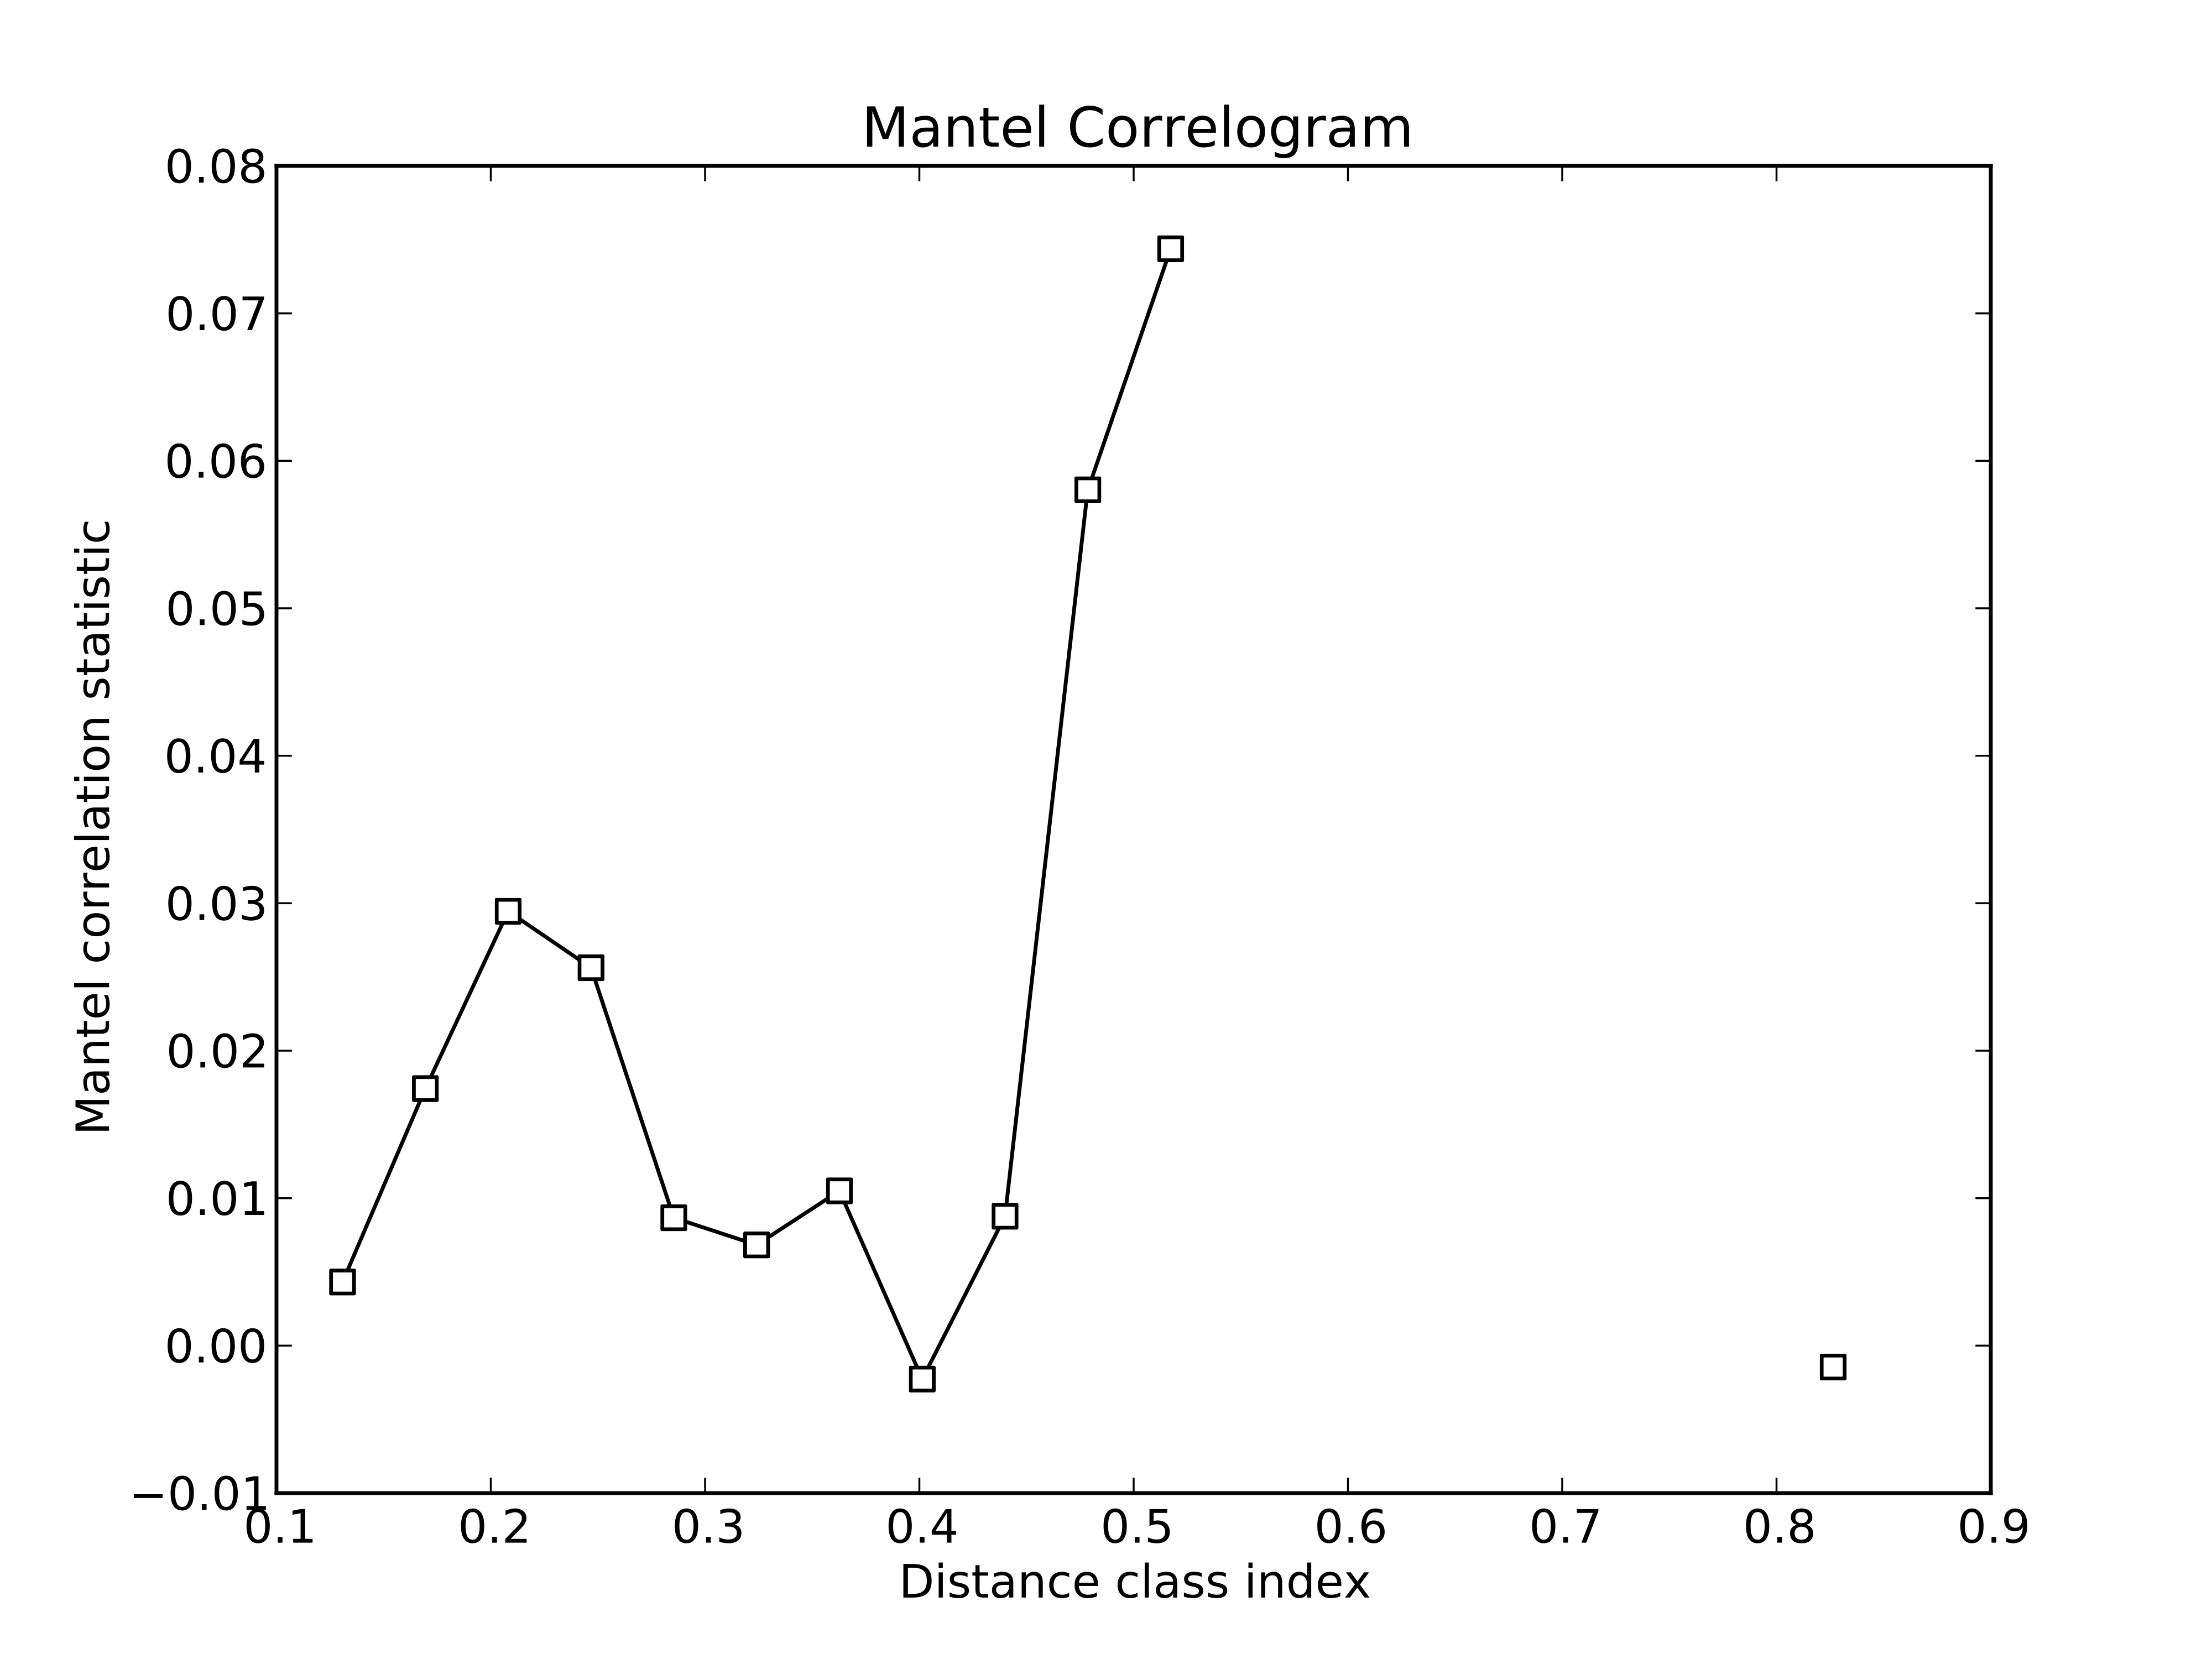
\includegraphics[width=0.75\columnwidth]{chapter_book_figures/Figure_10.jpg}
\caption[Mantel Correlogram showing the Mantel correlation statistics between unweighted Unifrac distance matrix and each class in the days after experiment started distance matrix]{\textbf{Mantel Correlogram showing the Mantel correlation statistics between unweighted Unifrac distance matrix and each class in the days after experiment started distance matrix.}
Classes in the second distance matrix are determined by Sturge's rule. White dots show non-significant relationship since black dots show significant ones.}
\label{bfigure10}
\end{figure}

The partial Mantel test is similar to the Mantel test, except that the analysis is
controlled by a third variable. When we compare the beta diversity distance matrix
with days after the experiment started by controlling by sampling date, we find the
same trend noted before (Partial Mantel test: p = 0.010). Samples collected
close in time have similar bacterial communities and this effect is independent of the date of collection.

Several visual and statistical tests have been implemented in \gls{qiime} in order to compare
between and within beta-diversity distances. Distance histograms are an easy way to
compare both types of distances graphically (make\_distance\_histograms.py). The output
is an html file that shows as many histograms as categories. It is very useful to compare
all-within “category” against all-between “category”, or the distribution of distances
within each group (Figure ~\ref{bfigure11}). Probably a more useful tool to compare these
beta-diversity distances is by means of box-plots (make\_distance\_boxplots.py, Figure ~\ref{bfigure12}).
The box-plot script generates a box-plot graph and performs a t-test. Box-plots showed that
there were no differences between the distances within mouse type and between types.
However, the statistical test shows highly significant differences (p $<$ 0.001) when comparing
within and between distances. Once again, we recommend caution and common sense when the
p-values are interpreted. It is likely to get a significant p-value, although a close
inspection of the box-plot reveals that standard error bars overlap. Basically this
result is due to the large number of comparisons: a small Student t-statistic
(obtained when differences between two data set are small) and these large degrees
of freedom may be highly significant (i.e. the two data set are very different) even
with conservative multiple test corrections (as Bonferroni).

\begin{figure}[htbp]
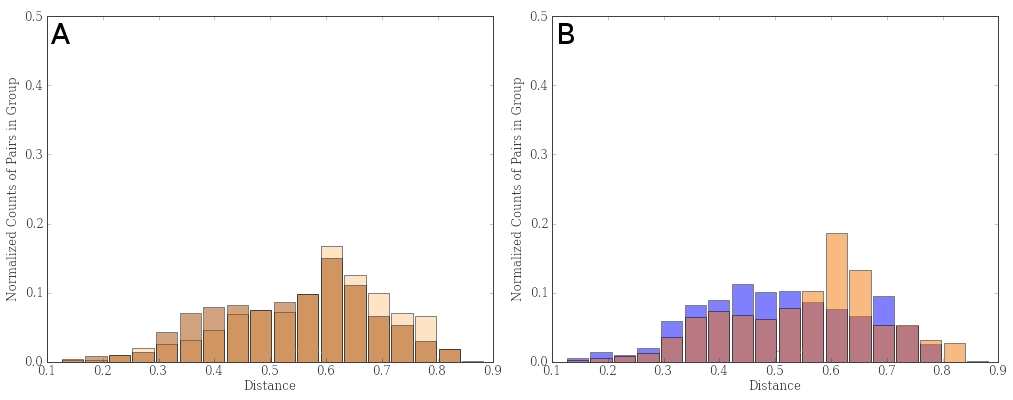
\includegraphics[width=\columnwidth]{chapter_book_figures/Figure_11.jpg}
\caption[Histograms of the example data set]{\textbf{Histograms of the example data set.}
(A) Histogram showing distribution of distances between (light brown) and within
(dark brown) mice gut microbiota taking into account both wild type and transgenic
mouse groups. (B) Distribution of within distances in gut bacterial community of wild
type mice (light orange) and transgenic ones (blue).}
\label{bfigure11}
\end{figure}

\begin{figure}[htbp]
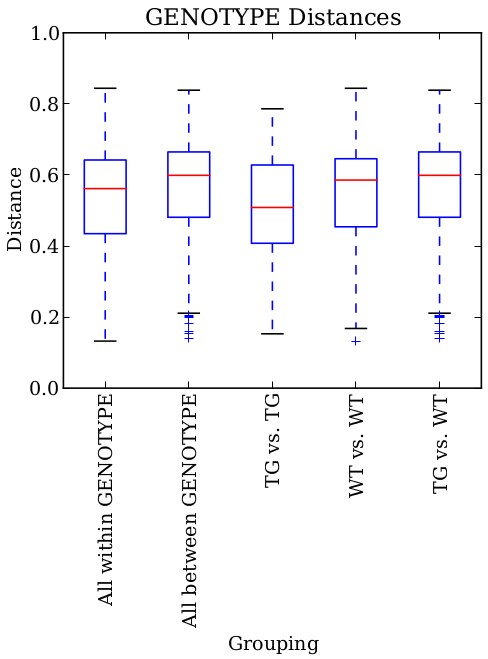
\includegraphics[width=0.75\columnwidth]{chapter_book_figures/Figure_12.jpg}
\caption[Box-plots of the unweighted UniFrac distances for bacterial gut microbiota in both mouse type (WT: wild type; TG: transgenic)]{\textbf{Box-plots of the unweighted UniFrac distances for bacterial gut microbiota in both mouse type (WT: wild type; TG: transgenic).}
“Within” distances represent distances within any of the two groups since “between” distances
show distances between both groups. “TG vs. TG” and “WT vs. WT” represent within distances in
transgenic and wild type groups respectively. Although averages are different, standard error overlaps
in all cases.}
\label{bfigure12}
\end{figure}

Other multivariate analyses provide additional powerful tools for exploring significant
relationships between the beta diversity distance matrix and factors or covariates.
compare\_categories.py offer different statistical tests, where ANOSIM and adonis are
usually employed. ANOSIM is a non-parametric statistical test that compares ranked
beta-diversity distances between different groups and calculates a p-value and a correlation
coefficient by permutation. Adonis partitions the variance in a similar way to the
ANOVA family of tests, specifically testing variation within a category is smaller
or greater than variation between categories. It calculates a pseudo F-value, a
p-value and a correlation coefficient (R2). Significant p-values must be
interpreted together with their R2 values to infer biological meanings from the results.
It is worth to mentioning here that PERMANOVA and adonis are similar statistical methods,
and usually provide equivalent results. However, PERMANOVA only allows categorical factors,
whereas both categorical and continuous variables may be used in adonis. Both ANOSIM and
adonis analyses indicate that bacterial communities in wild-type and transgenic mice
significantly differ from one another (ANOSIM: r = 0.134, p $<$ 0.001; adonis, r2 = 0.046, p $<$ 0.001).
However, the correlation coefficients are low, so the significant p-values need to be
interpreted cautiously because this result may not be biologically relevant.


\textbf{\gls{otu} networks.} Network-based analysis can sometimes be very useful for
displaying how \gls{otu}s are partitioned between samples, and how samples are related
each other, although we have found that this analysis only works well for datasets
in which the samples are not all equally connected. Networks are therefore a powerful
way for visually displaying certain large and complex datasets to emphasize similarities
and differences among samples. Network analyses are implemented in \gls{qiime} through the
script make\_otu\_network.py. This script generates the \gls{otu} network files to be
passed into Cytoscape \cite{Shannon2003} and statistics for those networks (specifically,
a bipartite graph in which nodes represent either \gls{otu}s or samples, and edges represent
a connection between an \gls{otu} and a sample (Ley et al., 2008)). Cytoscape is not wrapped
in the \gls{qiime} pipeline and it is run as a separate program. The files used by Cytoscape 2.8.2 are:
the real edge table (real\_edge\_table.txt) which contains the columns “from”, “to”, “eweight” and
“consensus\_lin”, among others dictated by the headers in the mapping file; and the real
node file (real\_node\_table.txt) which contains a node for each \gls{otu} and each sample in
the study. It uses the \gls{otu} file and the user metadata mapping file.

The visual output of this analysis is a clustering of samples according to their shared \gls{otu}s
(i.e. samples that share more \gls{otu}s cluster closer together, as do \gls{otu}s shared by more samples):
samples and \gls{otu}s are represented as dots in the space (“nodes”) and connected by lines (“edges”).
The degree to which samples cluster is based on the number of \gls{otu}s shared between samples, and this
is weighted according to the number of sequences within an \gls{otu}.

In the network diagram, both types of nodes, \gls{otu} nodes and sample nodes, can be
easily modified using Cytoscape's graphical user interface, with symbols such as
filled circles for \gls{otu}s and filled squares for samples. If an \gls{otu} is found within a
sample, both nodes are connected with a line (an edge). The nodes and edges can then
be colored to emphasize certain aspects of the data.

This method is not simply used for descriptive visualizations: the connections within
the network can also be analyzed statistically to provide support for the clustering patterns
displayed in the network. A G-test for independence is used to test whether sample nodes within
categories (such as within a genotype, in our example mouse study) are more connected within
than a group than expected by chance. Each pair of samples is classified according to whether
its members shared at least one \gls{otu}, and whether they share a category. Pairs are then
tested for independence in these categories (this asks whether pairs that share a category
also are equally likely to share an \gls{otu}). This statistical test can also provide support
for an apparent lack of clustering when it appears that a parameter is not contributing
to the clustering.

In our example dataset, mouse samples show some degree of clustering in the space
depending on whether the genotype is wild-type or transgenic (Figure ~\ref{bfigure13}).
These clusters in the network were significant different (G-test: p $<$ 0.001). Surprisingly,
bacterial communities of mice did not visually cluster by body site, although the statistical
test shows highly significant differences in samples from different body sites. These results
must be interpreted cautiously. The degrees of freedom in the statistical test depend on the
number of comparisons so, highly significant results might be obtained even when differences
between clusters are slight. In other cases, these differences are obvious and easy to interpret.
In the first application of this analysis in microbial ecology, the gut bacteria of a variety of
mammals was surveyed, and the network diagrams were colored according to the diets of the animals,
which highlighted the clustering of hosts by diet category (herbivores, carnivores, omnivores). In a
later meta-analysis of bacterial surveys across habitat types, the networks were colored in such a
way that the phylogenetic classification of the \gls{otu}s was highlighted: this analysis revealed
the dominance of shared Firmicutes in vertebrate gut samples versus a much higher diversity of
phyla represented amongst \gls{otu}s shared among environmental samples \cite{Ley2008}.

\begin{figure}[htbp]
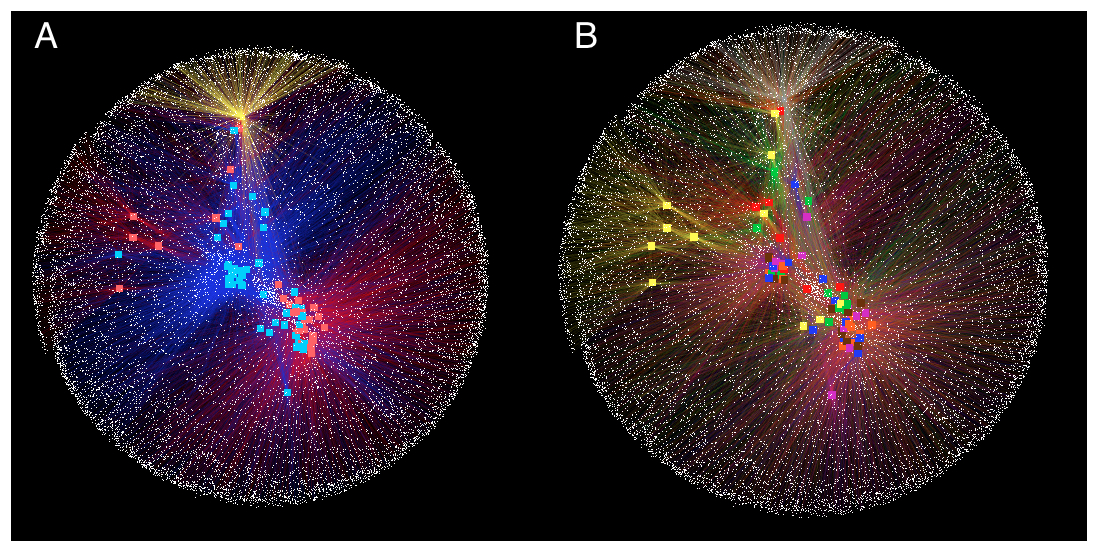
\includegraphics[width=\columnwidth]{chapter_book_figures/Figure_13.jpg}
\caption[\gls{otu}-Network bacterial community analysis applied in wild type and transgenic mice]{\textbf{\gls{otu}-Network bacterial community analysis applied in wild type and transgenic mice.}
(A) Network colored by genotype (wild type: blue; transgenic: red). Control sample (yellow dot) is
external in the network and several \gls{otu} are not shared with mice. Although we can see some degree of
clustering, discrimination by genotypes is difficult to assess. (B) Network colored by body site
(mouth: yellow; skin: in red; ileum: in blue; colon: in pink; cecum: in orange; feces: in brown;
and multi-tissue samples: in green). A control sample is colored in grey. There is no clear sample
clustering by body site, suggesting that there is not a core set of \gls{otu}s that differentiates one site from another.}
\label{bfigure13}
\end{figure}

This \gls{otu}-based approach to comparisons between samples provides a counterpoint to the
tree-based PCoA graphs derived from the UniFrac analyses. In most studies, the two
approaches reveal the same patterns. They can, however, reveal different aspects of the
data. The network analysis can provide taxonomic connections among samples in a visual manner,
whereas PCoA-UniFrac clustering can reveal sub-clusters that may be obscured in the network.
The principal coordinates can be pulled out individually and regressed against other metadata;
the network analysis can provide a visual display of shared versus unique \gls{otu}s. Thus, together
these tools can be used to draw attention to different aspects of a dataset.

\textbf{\gls{otu} heatmaps.} Another method to visualize the relationships between \gls{otu}s
and samples is the heatmap, which is widely used for other applications in molecular
biology \cite{Wilkinson2009}. This method was initially developed by Loua \cite{Loua1873}
to visualize population characteristics of 20 districts of Paris.

In our case, heatmaps can be used for exploratory analysis of microbiomes by mapping
abundance values to a color scale in a condensed, pattern-rich format, in which each
row corresponds to an \gls{otu} and each column corresponds to a sample. A good heatmap
graphic can generate hypotheses about sample and/or \gls{otu} clustering in the data, which can
then be followed up with additional more formal analyses. Two key structural aspects of a
heatmap graphic greatly affect whether it will reveal interpretable patterns: (1) the ordering
of the axes, and (2) the color scaling.

\gls{qiime} can create \gls{otu} heatmaps using two different scripts: make\_otu\_heatmap.py and
make\_otu\_heatmap\_html.py. The first script generates a heatmap in which \gls{otu}s are
represented in rows and samples in columns. \gls{otu}s and samples can be sorted and clustered
by the phylogenetic tree and by the UPGMA hierarchical clustering, respectively. However,
the visualizations of both trees (phylogenetic and hierarchical) in the final heatmap
are not currently implemented directly in \gls{qiime}, and these hierarchical displays must be
prepared using external software such as R. \gls{qiime} also supports sample clustering by a metadata
category if the user provides a mapping file. The samples will be clustered within each category
level using Euclidean UPGMA. The script sort\_otu\_table.py allows sorting the \gls{otu} table by a
category in the mapping file, allowing defining the order of the samples in the heatmap.
Figure ~\ref{bfigure14} shows the output of make\_otu\_heatmap.py. There we can see a drawback
to heatmaps: when the number of samples or \gls{otu}s included in the graphic is too high, the density
of the graphic can be overwhelming. Thus, we recommend that the \gls{otu} table be filtered to a
smaller number of samples (or categories) and taxa to identify the most important patterns,
as we will show later in this section.

\begin{figure}[htbp]
\includegraphics[width=0.75\columnwidth]{chapter_book_figures/Figure_14.jpg}
\caption[Heatmap of \gls{otu}s present in the different samples from transgenic and wild type mice]{\textbf{Heatmap of \gls{otu}s present in the different samples from transgenic and wild type mice.}
The intensity of black shows the abundance of certain \gls{otu} in each sample.
Both samples and \gls{otu}s are sorted by UPGMA tree and the \gls{otu} phylogenetic tree, respectively.}
\label{bfigure14}
\end{figure}

The second script (make\_otu\_heatmap\_html.py) creates an interactive \gls{otu} heatmap
from an \gls{otu} table (Figure ~\ref{bfigure15}). This script parses the \gls{otu} count table
and filters the table by counts per \gls{otu} (user-specified). It then converts the table
into a javascript array, which can be loaded into a web browser. The \gls{otu} heatmap
displays raw \gls{otu} counts per sample, where the counts are colored based on the
contribution of each \gls{otu} to the total \gls{otu} count present in the sample (blue:
contributes low percentage of \gls{otu}s to sample; red: contributes high percentage of
\gls{otu}s). This web application allows the user to filter the \gls{otu} table by number of
counts per \gls{otu}. The user also has the ability to view the table based on taxonomy
assignment. Additional features include: the ability to drag rows up and down by
clicking and dragging on the row headers; and the ability to zoom in on parts of
the heatmap by clicking on the counts within the heatmap.

\begin{figure}[htbp]
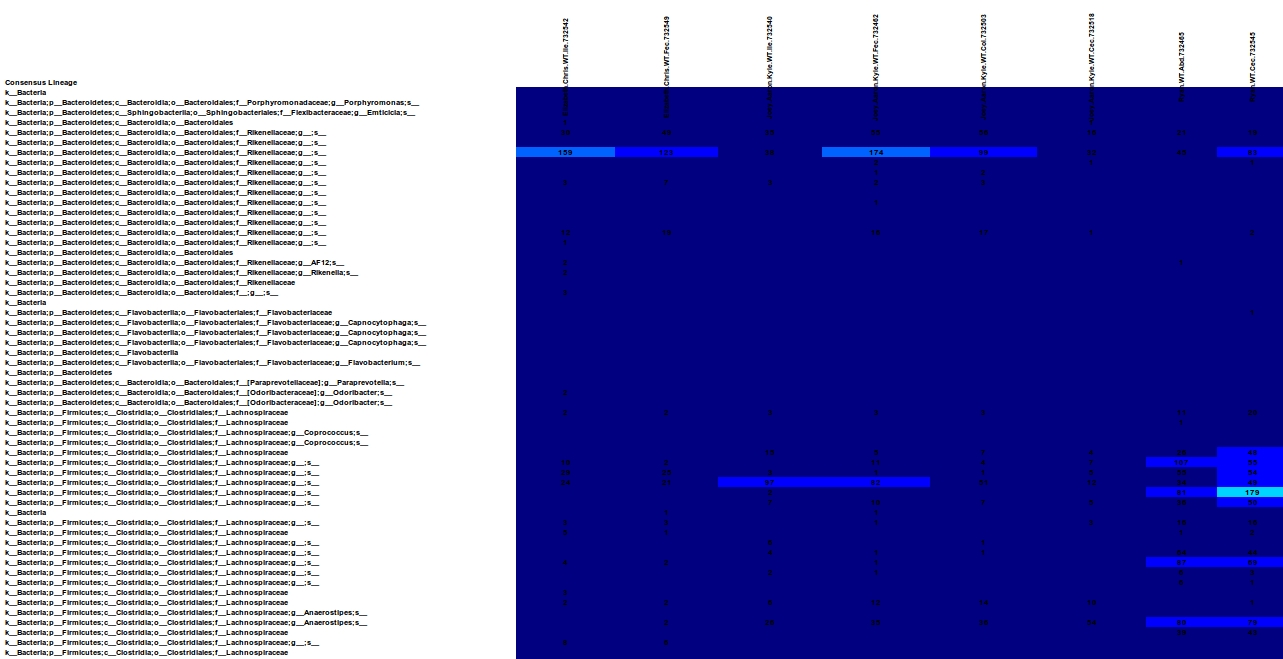
\includegraphics[width=0.75\columnwidth]{chapter_book_figures/Figure_15.jpg}
\caption[Interactive heatmap of \gls{otu}s present in the different samples from transgenic and wild type mice]{\textbf{Interactive heatmap of \gls{otu}s present in the different samples from transgenic and wild type mice.}
This visualization is a result of an HTML file that can be opened in any web browser.
The advantage of this heatmap is that it is easy to manipulate the abundance level for
coloring, or transpose samples and \gls{otu}s between columns and rows.}
\label{bfigure15}
\end{figure}

Improved \gls{otu} heatmap visualizations can be generated using the plot\_heatmap() command
in the phyloseq package for R \cite{McMurdie2013}. This package takes a similar approach
to NeatMap \cite{Rajaram2010}, in that it uses ordination results rather than hierarchical
clustering to determine the index order of each axis. For plot\_heatmap, the default color
scaling maps a particular shade of blue to a log transformation of abundance that generally
works well for microbiome data, although the user can select alternative transformations.

In this example, a key step was proper filtering of the data. We removed \gls{otu}s that appear in only a
few samples. The possible contribution to the graphic of these infrequent \gls{otu}s is limited, more often
contributing to “noise” that causes the heatmap to look dark, empty, and uninterpretable (see Figure ~\ref{bfigure14}).
We used a non-metric multidimensional scaling of the Bray-Curtis distance to determine the order of the \gls{otu}s and
samples. From this representation, it is possible to distinguish high-level patterns and simultaneously note the
samples and \gls{otu}s involved. For instance, all but a few of the mouth samples are in a cluster toward the middle of the
heatmap. One of the key features of this group is an obvious relative overabundance of three Firmicutes \gls{otu}s, which
are among the most abundant in this subset of the data. Similarly, another clear pattern is a distinction between a
group of wild type samples from various body sites on the left of the heatmap that appear to have higher proportions
of a number of different Firmicutes \gls{otu}s, as well as a few specific Bacteroidetes \gls{otu}s. This is distinct from the
largest cluster of samples on the right-hand side of the heatmap, in which many of the most-abundant \gls{otu}s are a
different subset of Bacteroidetes and Firmicutes \gls{otu}s. We also found it helpful to further pursue these high-level
patterns by splitting the data into Firmicutes-only and Bacteroidetes-only subsets, and then plotting new heatmaps
with finer-scale taxonomic labels. This required essentially the same commands and limited additional effort, well-tailored
for exploratory interactive analysis, much of which we have documented in Supplemental File 1.

Although heatmaps have been deployed widely in molecular biology, especially in protein expression studies, some of the
other displays we have discussed such as principal coordinates plots and taxonomy plots often provide more easily
interpretable results. However, summarizing relations between taxa through ordination plots or network analyses
have been shown to be powerful tools for highlighting similarities and differences among samples and taxa in our
\gls{otu} table, and a carefully constructed heatmap (though not, in most cases, the default output) can be a useful
guide to understanding and hypothesis generation.

\textbf{\gls{otu} category significance.} The experimental design of a microbial study will often involve
comparing two or more groups for differences in the abundance of \gls{otu}s; for example, are there taxa
that significantly differ between the control group and the experimental group? One way to assess
this question is to compare the relative abundances of each microbial member between the two groups.
This functionality is built into a script called otu\_category\_significance.py. We can test if there
are significant differences in \gls{otu} abundance between mouse genotypes either wild type (WT) or transgenic
(TG). We can assess differences between these groups using the following command:

\begin{lstlisting}[language=bash]
otu_category_significance.py \
 -i $PWD/diversity_analysis/open_ref/table_mc7205.biom \
 -m $PWD/IQ_Bio_16sV4_L001_map.txt \
 -o $PWD/open_ref_otu_categ_sig_output -c GENOTYPE \
 -s ANOVA
\end{lstlisting}

Here we run an ANOVA to assess the relative abundance of each taxon in the \gls{otu} table between our
two genotype groups. The output will be written to a user-specified file called otu\_cat\_sig.txt.
This document will list the \gls{otu} ID, the raw p-value, the Bonferonni corrected p-value, the False
Discovery Rate (FDR) p-value, as well as the relative average abundance for each of the groups in
the selected category (genotype in our case), and the \gls{otu} taxonomy string (if provided in the initial
\gls{otu} table). While many of these taxa may be significantly different between groups according to the
raw p-value, it is extremely important that only p-values that have been corrected for against multiple
comparisons, using either Bonferroni or FDR, be considered as significant. Many times a user's \gls{otu}
table will contain hundreds or thousands of \gls{otu}s, and thus a p-value is likely to reach significance
based solely on the large number of statistical comparisons being computed (for a probability threshold
of 0.05, 1 of 20 comparisons results significant just by chance). It is often very helpful to open the
.txt files produced by otu\_category\_significance.py in a spreadsheet so that columns can be sorted
according to p-values.

The otu\_category\_significance.py script also contains several other statistics for comparing groups.
The g-test can be used to determine if the presence or absence of a given taxa is significantly different
between groups, and can be specified by passing the option -s g\_test in the command. The user can also
run a paired t-test to determine whether there are taxa that significantly differ between two paired points.
For example, imagine the experimental design sampled a group of mice before and after a dietary intervention.
Using the paired-t statistic in otu\_category\_significance.py would then compare each mouse's after timepoint
to the before timepoint, and test for differences that were consistent across mice, rather than grouping all
the before and after timepoints together. For continuous variables, \gls{qiime} can calculate the Pearson correlations
of \gls{otu} abundance with those variables. \gls{qiime} is also capable of longitudinal data analysis, which is suitable
for the samples tracking the same subjects at multiple points in time, e.g., the oral microbiota of 6 persons
after meals in a day. Specifically, longitudinal Pearson correlation can be calculated, accounting for intra-subject
correlation of measurements.

\textbf{Machine learning.} \gls{qiime} can also take advantage of several machine learning algorithms to solve
two important issues in high-throughput metagenomic studies: correction of mislabeling, and quantifying
sample contamination.

This mislabeling problem is an increasing issue as the number of processed and pooled sequences
increases \cite{Knights2011Mislabel}. This mislabeling can be addressed using supervised classifiers,
a machine learning technique that is able to fix incorrect metadata. \gls{qiime} uses the random forest \cite{Breiman2001}
supervised classifier implemented in R \cite{Liaw2002} to recover the mislabeled samples by training the
classifier with the relative abundance taxa \cite{Knights2011SupClass}. Knights et al. \cite{Knights2011Mislabel}
shows that this approach can even recover up to 30-40\% mislabeled samples when the biological patterns are especially clear.

This same technique can be also applied to find taxa that play a key role in differentiating groups of samples, as
is done in \gls{otu} category significance. However, the difference between \gls{otu} category significance and the machine
learning technique is the type of model the construct. While the \gls{otu} category significance creates an explanatory
model (i.e. it gives a model that best fits the current dataset), the machine learning technique creates a predictive
model \cite{Knights2011SupClass}.That is, it creates a model that is able to generalize future data, minimizing the
expected prediction error.

Since the supervised learning trains a classifier, it is important to provide useful predictors (\gls{otu}s in our case).
Thus, it is highly recommended to filter the input \gls{otu} table to remove those \gls{otu}s that are present in few samples
(e.g. $<$ 10 samples). As in previous analyses, a rarified \gls{otu} table should be used, so that artificial diversity
induced due to different sampling effort is removed. In our example dataset, we can use the subsampled \gls{otu} table
generated for previous analyses and remove the low-abundance \gls{otu}s:

\begin{lstlisting}[language=bash]
filter_otus_from_otu_table.py \
 -i $PWD/diversity_analysis/open_ref/table_mc7205.biom \
 -o $PWD/diversity_analysis/open_ref/otu_table_filtered10.biom \
 -s 10
\end{lstlisting}

Running the following command, will run the supervised learning algorithm using the GENOTYPE
category and 10-fold cross-validation, providing mean and standard deviation of errors:

\begin{lstlisting}[language=bash]
supervised_learning.py \
 -i $PWD/diversity_analysis/open_ref/otu_table_filtered10.biom \
 -m $PWD/IQ_Bio_16sV4_L001_map.txt -c GENOTYPE \
 -o $PWD/open_ref_supervised_learning_output -e cv10
\end{lstlisting}

This script will store several files on the output folder. The most important file is summary.txt:

\begin{lstlisting}[language=bash]
cat $PWD/open_ref_supervised_learning_output/summary.txt
Model Random Forest
Error type 10-fold cross validation
Estimated error (mean +/- s.d.) 0.23373 +/- 0.15058
Baseline error (for random guessing) 0.42308
Ratio baseline error to observed error 1.81011
Number of trees 500
\end{lstlisting}

The important information in this file is the Ratio baseline error to observed error, which shows the
ratio between the expected error of the random forest classifier and the expected error of a classifier
that always guesses the most abundant class (Baseline error). Our recommendation is that a ratio of at
least 2 shows a good classification. In our example data set, this value is 1.81011, which is close to 2
but not enough to be considered a good classification.

The contamination quantification problem is addressed in \gls{qiime} using SourceTracker \cite{Knights2011}. Given a
list of known source environments and a sink (or set of sinks) environment(s), SourceTracker uses a Bayesian
approach jointly with Gibbs sampling to predict the quantity of taxa that each source, or an unknown source,
contributes to the taxa that makes up the sink environment. For a more detailed description of the algorithm,
see Knights et al. \cite{Knights2011}.

The first step to use SourceTracker in \gls{qiime} is to modify the mapping file of our example dataset and add two
columns: SourceSink and Env. The SourceSink column tells SourceTracker which sample is a source and which
sample is a sink, while the Env column provides the environment. In our example, we have defined samples from
mouth, ileum, cecum, colon, fecal pellet and skin as sources and the whole mouse homogenization as a sink. In
the Env column we have defined the environments as the body site (mouth, ileum, cecum, colon, feces, skin and homogenization).

As a machine learning algorithm, SourceTracker needs useful \gls{otu}s (predictors) as inputs for training the algorithm.
Here, we will use the same \gls{otu} table as used for the supervised\_learning.py script. However, SourceTracker does not
yet accept BIOM tables, so we have to transform them into to a tab-delimited \gls{otu} table (note that this table can also
be opened in Excel or other popular tools):

\begin{lstlisting}[language=bash]
convert_biom.py \
 -i $PWD/diversity_analysis/open_ref/otu_table_filtered10.biom \
 -o $PWD/diversity_analysis/open_ref/otu_table_filtered10.txt -b
\end{lstlisting}

Then, we can call SourceTracker using the following command (the \$SOURCETRACKER\_PATH variable should be defined if
you have successfully install SourceTracker):

\begin{lstlisting}[language=bash]
R --slave --vanilla --args \
 -i $PWD/diversity_analysis/open_ref/otu_table_filtered10.txt \
 -m $PWD/IQ_Bio_16sV4_L001_map_ST.txt \
 -o $PWD/open_ref_sourcetracker_output \
 < $SOURCETRACKER_PATH/sourcetracker_for_qiime.r
\end{lstlisting}

The output from the SourceTracker algorithm is a set of pdf files that shows the mixture of
the sources that makes up the sink (see Figure ~\ref{bfigure17}).

\begin{figure}[htbp]
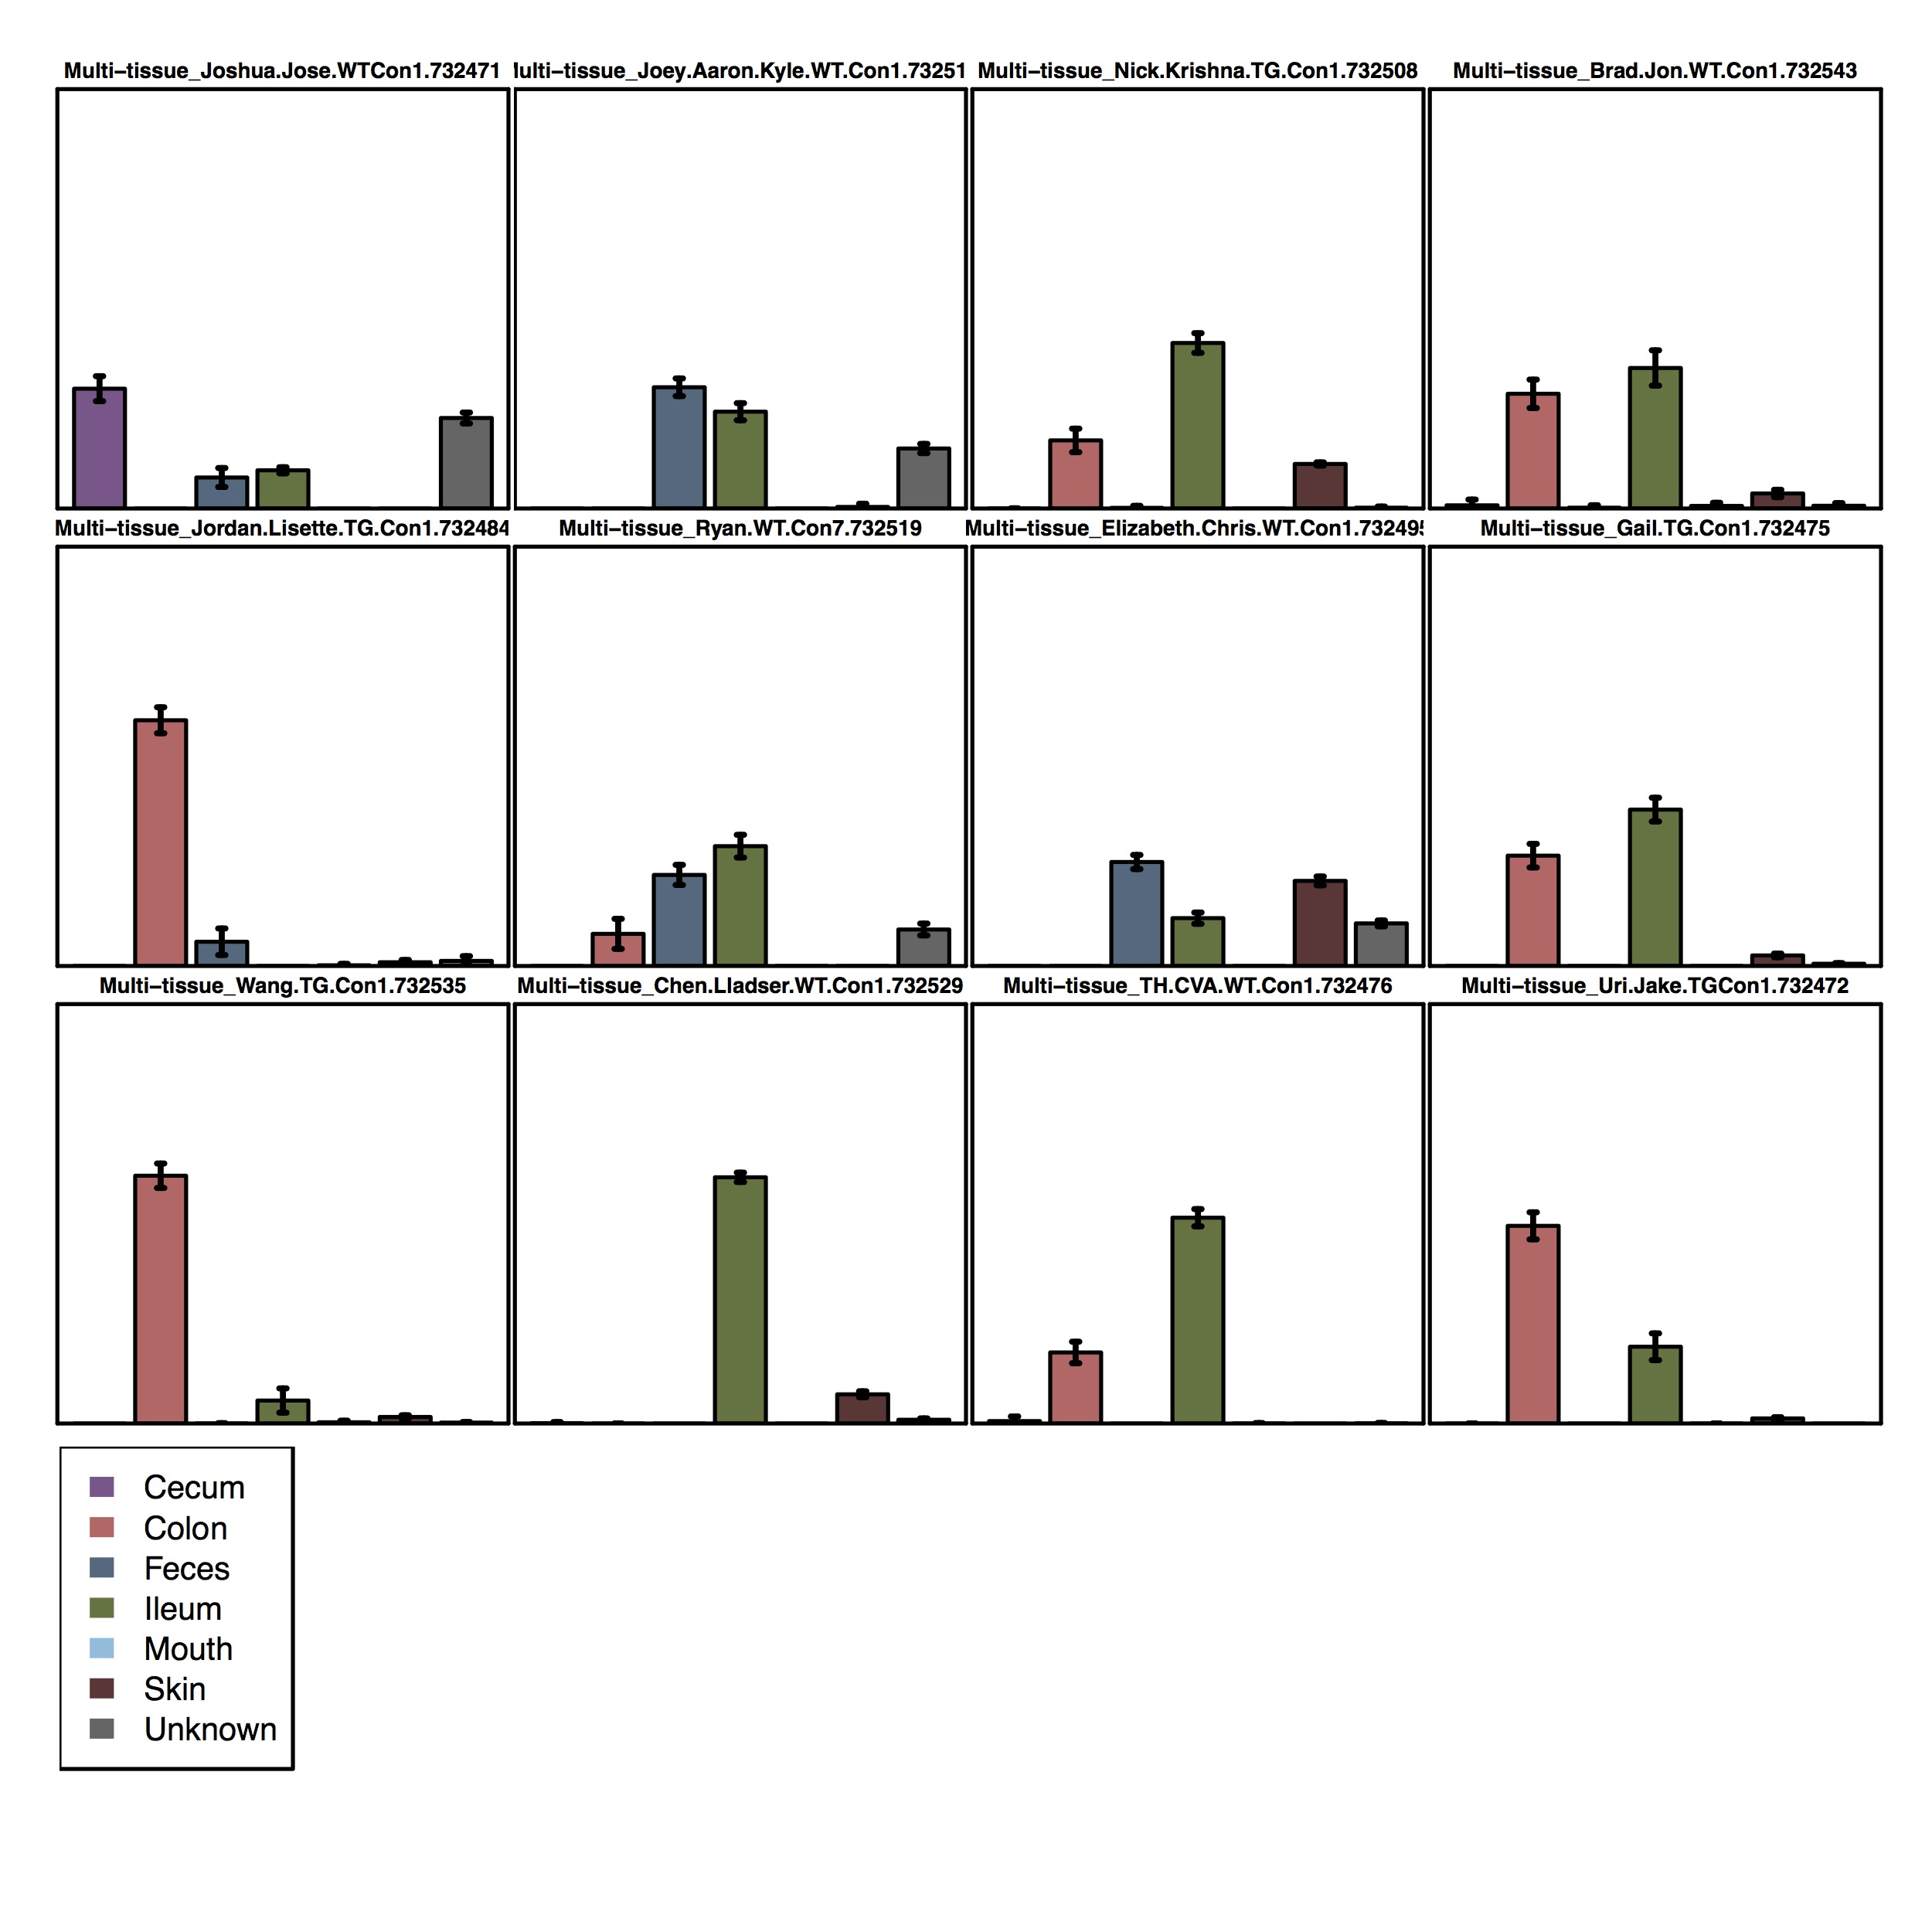
\includegraphics[width=\columnwidth]{chapter_book_figures/Figure_17.jpg}
\caption[SourceTracker output showing a bar plot for each sink (mouse) present in the dataset]{\textbf{SourceTracker output showing a bar plot for each sink (mouse) present in the dataset.}
Each bar is a potential source (body site) and the height of each bar represents the percentage of
taxa the source contributes to the taxa in the sink. The advantage of this visualization over the other
two (area and pie chart) is that it shows error bars that allow to see the variance of the prediction.}
\label{bfigure17}
\end{figure}

\textbf{Procrustes analysis.} When we want to compare samples in PCoA space that
were processed in different ways, such as: different ribosomal RNA subunits, primer sets,
or algorithmic choices for processing, we can use Procrustes analysis \cite{Gower1966, Muegge2011, Vinten2011}.
Procrustes analysis is a statistical shape algorithm that allows us to compare different distributions by
rescaling and applying a rotation matrix; this is, if the group of samples we are have the same shape but
in different size or orientation the algorithm will resize and rotate them to make the shapes fit. As an example,
we present the results of comparing the different \gls{otu} picking algorithms, where we can see that even as the number
of \gls{otu} clusters change the distribution described is similar with a confidence of MC p-value: 0.00 and M2: 0.097 for
closed-reference vs. de novo, and MC p-value: 0.00 and M2: 0.035 for closed-reference vs. open reference.
Both cases used the first three axes (i.e. the axes displayed in the plot), and 100 repetitions, Figure \ref{bfigure18}.
To generate these plots we ran these commands:

\begin{lstlisting}[language=bash]
transform_coordinate_matrices.py \
 -i $PWD/diversity_analysis/closed_ref/bdiv_even7205/\
 unweighted_unifrac_pc.txt,$PWD/diversity_analysis/denovo/\
 bdiv_even7205/unweighted_unifrac_pc.txt \
 -r 100 -o $PWD/procrustes/closed_ref-denovo

compare_3d_plots.py \
 -i $PWD/procrustes/closed_ref-denovo/pc1_transformed.txt,\
 $PWD/procrustes/closed_ref-denovo/pc2_transformed.txt \
 -o $PWD/procrustes/closed_ref-denovo/plot \
 -m $PWD/IQ_Bio_16sV4_L001_map.txt

transform_coordinate_matrices.py \
 -i $PWD/diversity_analysis/closed_ref/bdiv_even7205/\
 unweighted_unifrac_pc.txt,$PWD/diversity_analysis/open_ref/\
 bdiv_even7205/unweighted_unifrac_pc.txt \
 -r 100 -o $PWD/procrustes/closed_ref-open_ref

compare_3d_plots.py \
 -i $PWD/procrustes/closed_ref-open_ref/pc1_transformed.txt,\
 $PWD/procrustes/closed_ref-open_ref/pc2_transformed.txt \
 -o $PWD/procrustes/closed_ref-open_ref/plot \
 -m $PWD/IQ_Bio_16sV4_L001_map.txt
\end{lstlisting}

\begin{figure}[htbp]
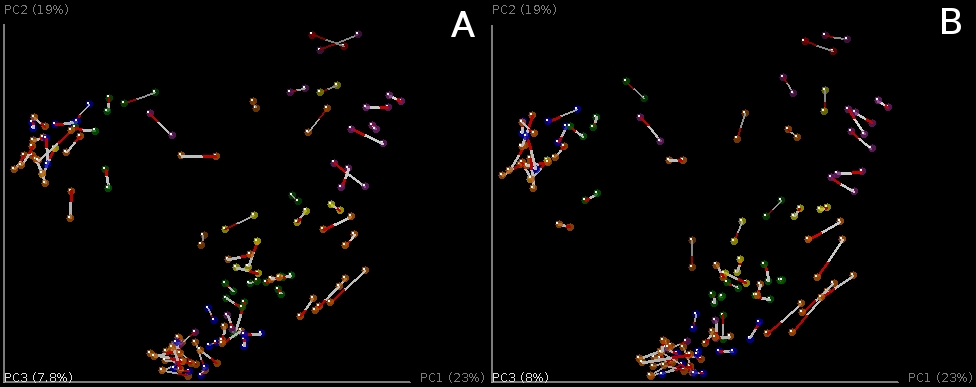
\includegraphics[width=\columnwidth]{chapter_book_figures/Figure_18.jpg}
\caption[Procrustes analysis of different picking algorithms, where we can see that different \gls{otu} clustering methods yield similar PCoA distributions]{\textbf{Procrustes analysis of different picking algorithms, where we can see that different \gls{otu} clustering methods yield similar PCoA distributions.}
PCoA plots are colored by BODY\_HABITAT. A) Comparing samples with clusters picked
using the de novo picking protocol against the closed-reference. B) Comparing
samples with clusters picked using the open-reference picking protocol against the closed-reference.}
\label{bfigure18}
\end{figure}

\textbf{SitePainter.} Spatial data poses unique challenges, and the types of statistical analyses
described above often obscure spatial patterns \cite{Gevers2012, Hewitt2013}.
SitePainter \cite{Gonzalez2012SitePainter} is a web-based tool that creates images representing the
geographical (spatial) distribution of our samples, and then color them based on taxonomy summaries
(defining which taxa occur where), and PCoA axes (defining how similar the patches are along the principal axes).

To create a new image we suggest using Adobe Illustrator, Inkscape or SitePainter. This list is in descending
order of usability. In any of these tools, we need to create a \gls{svg} image that has closed paths, ellipsoids
and rectangles for any path that we want to color; and open paths, lines or text for those that we want SitePainter
to ignore. The latter are useful for static images and give a nice background for the image. Note that \gls{svg}
images are text files, so they can be opened in any graphics program in the list above, or in any text editor.
The difference between an open and closed paths is that the element in has a letter z at the end of the definition
of the lines of the path, so, for example, \texttt{<path d=“M 10 10 L 30 10 L 20 30 z”>} is a closed path but
\texttt{<path d=“M 10 10 L 30 10 L 20 30”>} is an open one.

There are two main \gls{qiime}-generated inputs that should be loaded into SitePainter: taxa summaries and
\gls{mds} technique results, including NMDS and PCoA. To exemplify the creation and usage of images in
SitePainter, we will filter the \gls{otu} table and the beta diversity file to only have one mouse.
Filtering and summarizing the \gls{otu} table:

\begin{lstlisting}[language=bash]
filter_samples_from_otu_table.py
 -i $PWD/diversity_analysis/open_ref/bdiv_even7205\
 /table_mc7205_even7205.biom \
 -m $PWD/IQ_Bio_16sV4_L001_map.txt \
 -o $PWD/forSitePainter/otu_table_Gail.biom \
 -s ‘GROUP:Gail’

summarize_taxa.py \
 -i $PWD/forSitePainter/otu_table_Gail.biom \
 -o $PWD/forSitePainter/taxa_sum -t
\end{lstlisting}

Filtering the beta diversity file and then recalculating PCoA is necessary every time we add or remove
samples of our analyses, because PCoA results depend on the samples included in the analysis. Thus it is
not sufficient to simply remove samples from PCoA results calculated on a larger set of samples:

\begin{lstlisting}[language=bash]
filter_distance_matrix.py \
 -i $PWD/diversity_analysis/open_ref/bdiv_even7205\
 /unweighted_unifrac_dm.txt \
 -m IQ_Bio_16sV4_L001_map.txt \
 -o $PWD/forSitePainter/unweighted_unifrac_dm.txt \
 -s ‘GROUP:Gail’

principal_coordinates.py \
 -i $PWD/forSitePainter/unweighted_unifrac_dm.txt \
 -o $PWD/forSitePainter/unweighted_unifrac_pc.txt
\end{lstlisting}

Then we create an image in Adobe Illustrator that represents the mice and its gastrointestinal tract,
Figure ~\ref{bfigure19}-A. Once this figure is created and saved in \gls{svg} format (this example uses
version 1.1 of \gls{svg}), we open the image in any text editor and replace any letter ‘z’ with nothing;
this will destroy all the closed paths and will facilitate manipulation in SitePainter.

\begin{figure}[htbp]
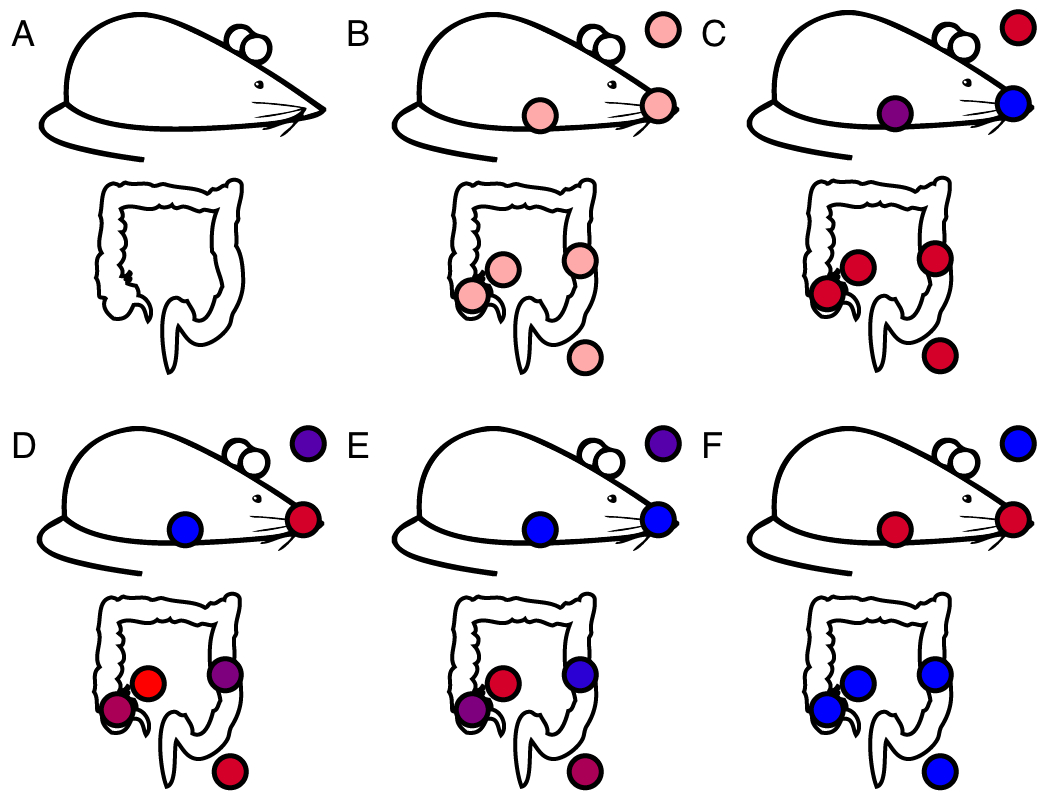
\includegraphics[width=0.75\columnwidth]{chapter_book_figures/Figure_19.jpg}
\caption[Image representing the mouse and its gastrointestinal tract]{\textbf{Image representing the mouse and its gastrointestinal tract.}
A) Raw image without samples. B) Image in SitePainter with samples. C-D)
PCoA axis 1 and 2, in red high values, in blue low values, similar colors represent
similar communities. E-F) Taxonomic distributions of (E) Betaproteobacteria and (F)
Gammaproteobacteria, in red high abundance, in blue low abundance.}
\label{bfigure19}
\end{figure}

Now, we can open this image in SitePainter by clicking on the pencil/flower image on
the right corner, choosing “Open Image”, and select our file. Then we add the places
that we want to color using the rectangle or ellipsoid tool, Figure ~\ref{bfigure19}-B.
Now we need to make our samples in the image match the names of the sample names from our
files; for this we need to click on “\texttt{Elem. -> Click to update}” on the right menu,
this will show us the current sample names in the image; then, we double click on each one
and change the name to make it match the sample name in the mapping file. Note that
SitePainter does not accept sample names with dots (.), so if the sample name has this character,
we need to replace it with an underscore (\_). We do not need to change the \gls{qiime} files, as this
will happen automatically in SitePainter. When we hover over each name, the sample will change color,
facilitating the identification of the image we are selecting. If different sites have the same name,
they will be colored with the same value from the \gls{qiime} output files.

The final step is to load the resulting \gls{qiime} files. To do this, we use the Metadata loader
on the top left of the menu. This opens the file. We then move the right menu to the “Meta.”
tab. Here we can select which column we want to use for coloring, and then click “Color elements”,
to select more, Figure ~\ref{bfigure19}-C-F. For detailed instructions about changing colors and
other details visit SitePainter's website \footnote{\url{http://sitepainter.sourceforge.net/tutorials/index.html}}.

\subsection{Other features}
\subsubsection{Testing linear gradients, including time series analysis}

Recent microbiome surveys have started integrating gradients (commonly over time) in their study design.
We will discuss a first and general approach for those cases, using the Moving Pictures of the Human
Microbiome Dataset \cite{Caporaso2011}, where two subjects were sampled daily for up to 396 days in three
different body sites (sebum, saliva and feces). Note that the mouse dataset that we use as a primary example
lacks a natural temporal ordering in the study design, so we can not use it as an example for this analysis.

PCoA plots provide a snapshot about the relative communities of many samples condensed in a single figure.
However, coloring the points in PCoA space according to a color gradient can be very difficult to understand.
A first approach in this case is to connect the samples belonging to the same subject/treatment subsequently
sorted using the values in the gradient, i.e. one timepoint after the other (see Figure ~\ref{bfigure20} b).
An interactive plot like this can be generated using the following command:

\begin{lstlisting}[language=bash]
make_3d_plots.py \
 -i $PWD/moving_pictures/unweighted_unifrac_pc.txt \
 -m $PWD/moving_pictures/merged_columns_mapping_file.txt \
 -o $PWD/moving_pictures/vectors \
 --add_vectors=BODY_SITEHOST_SUBJECT_ID,DAYS_SINCE_EPOCH
\end{lstlisting}

\begin{figure}[htbp]
\includegraphics[width=\columnwidth]{chapter_book_figures/Figure_20.jpg}
\caption[Beta diversity plots for the moving pictures dataset using unweighted UniFrac as the dissimilarity metric]{\textbf{Beta diversity plots for the moving pictures dataset using unweighted UniFrac as the dissimilarity metric.}
(a) PCoA plot colored by the body site and subject. (b) PCoA plot colored by the body
site and subject with connecting lines between samples. Note in (b) that these lines
allow us to track the individual body sites with a different approach.}
\label{bfigure20}
\end{figure}

An important thing to note here is that because we want to track each of the three
body-sites (SampleTypes) for the two subjects (Subject), we need a column in our
mapping file that allows us to make that distinction. Hence we need to concatenate
those two columns in our metadata mapping file using an external spreadsheet editor or
another tool. Also note that the gradient used is a category named DAYS\_SINCE\_EPOCH
(i.e. the number of days since January 1, 1970). The idea here is to have a common
reference for the collection date of each of the samples.

Although a visualization like the one created in the previous example is often sufficient,
replacing one of the axes in the PCoA plot with the data explaining the gradient provides a
different insight into the analyzed data (See Figure ~\ref{bfigure21}).

\begin{figure}[htbp]
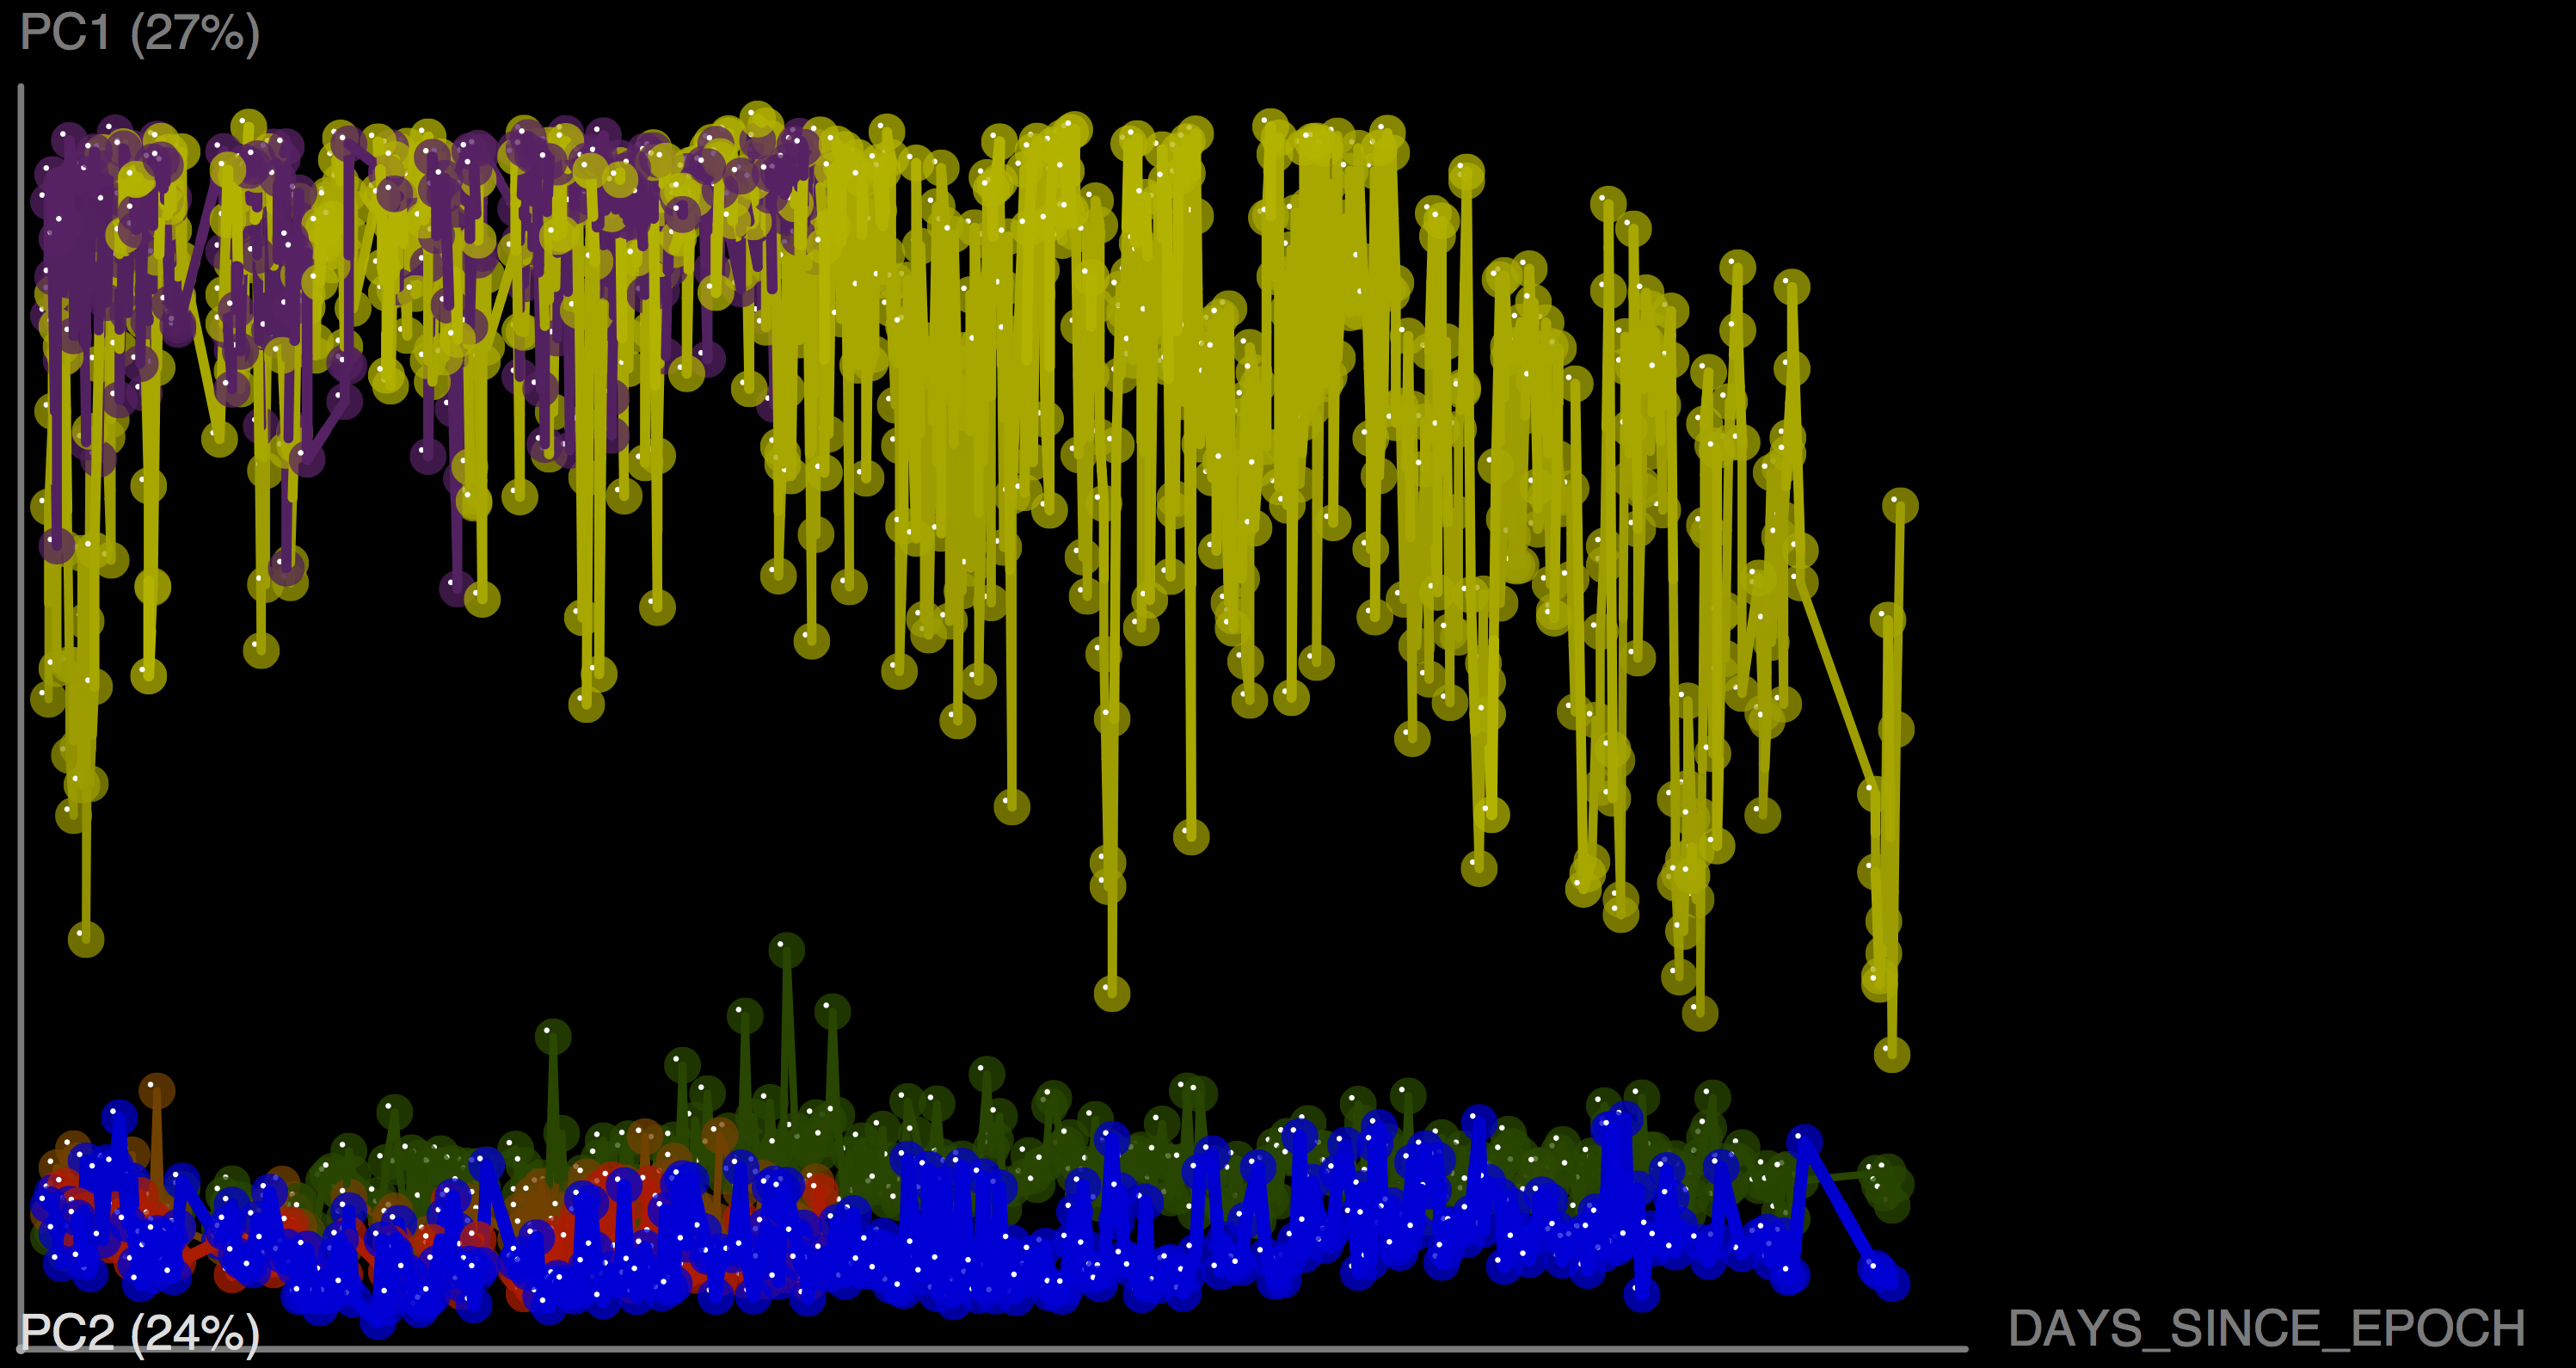
\includegraphics[width=0.75\columnwidth]{chapter_book_figures/Figure_21.jpg}
\caption[Three dimensional plots in which two of the axes are PC1 and PC2 and the other is the day when that sample was collected in reference to the epoch time]{\textbf{Three dimensional plots in which two of the axes are PC1 and PC2 and the other is the day when that sample was collected in reference to the epoch time.}
Although this is not explicitly a beta diversity plot, this representation allows differentiation of the individual trajectories over time.}
\label{bfigure21}
\end{figure}

\begin{lstlisting}[language=bash]
make_3d_plots.py \
 -i $PWD/moving_pictures/unweighted_unifrac_pc.txt \
 -m $PWD/moving_pictures/merged_columns_mapping_file.txt \
 -o $PWD/moving_pictures/vectors \
 --add_vectors=BODY_SITEHOST_SUBJECT_ID,DAYS_SINCE_EPOCH \
 -a DAYS_SINCE_EPOCH
\end{lstlisting}

These visual representations can often identify meaningful patterns. To statistically
support these assertions, one-way analysis of variance (ANOVA) can be used over the
values grouped by a category of interest. In a case where user wants to test for
independence between the variation of one group of trajectories and another,
this command could be used:

\begin{lstlisting}[language=bash]
make_3d_plots.py \
 –i unweighted_unifrac_pc.txt \
 –m mapping_file.txt –o vectors \
 –add_vectors=SampleTypeAndSubject,days_since_epoch \
 –a days_since_epoch --vectors_algorithm avg \
 --vectors_path anova_stats.txt
\end{lstlisting}

\subsubsection{Processing 454 data}

We have described the recommended workflow for conducting microbial community analysis on an
Illumina MiSeq dataset. However, \gls{qiime} can also perform microbial community analysis on the
454 platform. The main advantage of 454 over Illumina is that 454 generates longer sequences,
which can allow a better taxonomy assignment. However, the 454 technology produces fewer reads per
dollar, or per sequencing run \cite{Kuczynski2011}.

The 454 processing workflow differs from the Illumina workflow in the sequence preprocessing.
In this case, the output file from the sequencing facility is a fasta file containing the reads,
and a quality score file which contains the score for each base in each sequence included in the FASTA file.
In this case, the command used for the 454 preprocessing is split\_libraries.py:

\begin{lstlisting}[language=bash]
split_libraries.py \
 -m Fasting_map.txt -f Fasting_Example.fna \
 -q Fasting_Example.qual -o slout
\end{lstlisting}

Similarly to the Illumina processing, this script also performs a quality filtering.
In this case, the quality filtering is based on cut-offs for sequence length, end-trimming
or minimum quality score. However, to successfully remove the read artifacts, a
denoising process has to be performed \cite{Reeder2010} to reduce the impact of homopolymer
runs (runs of the same base). The 454 denoising process is a slow, computationally intensive
problem that does not scale to large datasets, as it is based on flowgram clustering \cite{Quince2011}.

\textbf{Variable length barcodes} Variable-length barcodes are used for two reasons:
to make the number of flows (rather than the number of bases) constant \cite{Frank2009},
or to stagger the reads to reduce bad signal from low complexity at a given position in
the set of amplicons being sequenced. This approach is not recommended today because such
samples are not easily demultiplexed, and there is checksum, like Hamming or Golay, that
allows error-correction and improved sample assignment \cite{Hamady2008}. However,
the \gls{hmp} used variable length barcodes to identify their samples within sequencing runs.
Thus, \gls{qiime} allows demultiplexing such files by using the parameter -b in split\_libraries.py, as follows:

\begin{lstlisting}[language=bash]
split_libraries.py \
 -m map_file_with_variable_length_barcodes.txt \
 -f your_fna.fna -q your_qual.qual \
 -o split_library_output_variable_length/ \
 -b variable_length
\end{lstlisting}

\subsubsection{18S rRNA gene sequencing}
\gls{qiime} can be also used to perform analysis on 18S \gls{rrna} gene sequence data
(in eukaryotes), as well as other markers such as \gls{its}. The main difference
between performing analyses with 18S \gls{rrna} gene data instead of 16S \gls{rrna} gene
data (or \gls{its} data) is the reference database used for \gls{otu} picking,
the taxonomic assignments and the template-based alignment building, since it must
contain eukaryotic sequences.

The recommended database to use as a reference for 18S \gls{rrna} sequences is
the Silva database \cite{Quast2013}. At the time of writing, the most recent
\gls{qiime}-compatible Silva database is the 108 release. Since this database contains
the three domains of life, it can be used as a reference for 18S \gls{rrna} data sets.

When conducting studies mixing 18S \gls{rrna} data and 16S \gls{rrna} data, you
should take into account that picking \gls{otu}s against the Silva database will assign
taxa to all three domains of life. In this case, it is recommended to split the
\gls{otu} table by domain, generating an \gls{otu} for each domain (Archaea, Bacteria and Eukarya).
At this point, each of these tables can be used in downstream analysis in the same
way as performed for 16S \gls{rrna} data.

\subsubsection{Shotgun metagenomics}

Shotgun metagenomics is also supported in \gls{qiime}, although it is still experimental
and it should be used at the user's own risk. Currently, the \gls{qiime} team recommends
the blat method \cite{Kent2002} for searching nucleic acid sequence reads in a
reference database, although usearch \cite{Edgar2010} is also supported. The main
reason for preferring blat against usearch is that protein reference database often
require 64-bit applications, and blat is free of charge, while the 64 bit version of usearch is not.

There are many reference databases (IMG, KEGG, M5nr, among others), and they all
supported by \gls{qiime}, since the user only needs to supply a single fasta file containing
the sequence records. The command that \gls{qiime} provides for mapping reads against the
reference database is map\_reads\_to\_reference.py, and it can be performed in parallel
using the parallel\_map\_reads\_to\_reference.py script.

\subsubsection{Support for QIIME in R}

First published in 1996, “R” is an integrated software application and programming
language designed for interactive data analysis (R Core Team). It is available for Linux,
Mac OS, and Windows free of charge under an open-source license (GPL2). Since its inception,
R has found a niche as a tool for interactive statistical analysis through functional programming.
Primary investigation and inference are performed by writing a series of repeatable commands as
“scripts” that can be recorded and published. This paradigm lends itself well to reproducible
research, and is enhanced substantially by R's integration with tools for literate programming
such as Sweave \cite{FriedrichLeisch2002}, knitr \cite{Xie2013}, and R markdown
\footnote{\url{http://CRAN.R-project.org/package=markdown}}, as well as data graphics. There are thousands
of free and open-source extensions to R (“packages”) available from the main R repository, CRAN,
further organized by volunteer experts into 31 task “views” (which are in fact workflow inventories).
Among these are dedicated package lists relevant to microbiome data, including phylogenetics, clustering,
environmetrics, machine learning, multivariate and spatial statistics, as well as a separate reviewed and
curated repository dedicated to biological statistics called Bioconductor (over 600 packages).

At present, support for \gls{qiime} in R is predominantly achieved through a package called “phyloseq” \cite{McMurdie2013}
dedicated to the reproducible analysis of microbiome census data in R. phyloseq defines an object-oriented data class
for the consistent representation of related (heterogenous) microbiome census data that is independent of the sequencing-
or \gls{otu}-clustering method (storing \gls{otu} abundance, taxonomy classification, phylogenetic relationships, representative
biological sequences and sample covariates). The package supports \gls{qiime} by including functions for importing data
from biom-format files derived from more recent versions of \gls{qiime} (import\_biom) as well as legacy \gls{otu}-taxonomy delimited
files (import\_qiime and related user accessible subfunctions). Later editions of phyloseq ($>$1.5.15) also include an
API for importing data directly from the microbio.me/qiime data repository. In all cases, these API functions
return an instance of the “phyloseq” class that contains the available heterogenous components in “native” R classes.
phyloseq includes a number of tools for connecting with other microbiome analysis functions available in other R packages,
as well as its own functions for flexible graphics production built using ggplot2 \cite{Wickham2009}, demonstrated
in supplemental files and online tutorials. For researchers interested in developing or using methods not directly
supported by phyloseq, nor its data infrastructure, the biom-format specific core functions in phyloseq have been
migrated to an official API in the biom-format project as an installable R package called “biom”, now released on
CRAN. This also includes some biom-format specific functionality that is beyond the scope of phyloseq, though support
for \gls{qiime} is still likely best achieved using phyloseq.

As with some of the earlier examples of \gls{qiime} commands with corresponding output and figures, in this section we
have included some key R commands potentially useful during interactive analysis in the R environment. For simplicity,
show only results related to the open-reference \gls{otu} data, stored in an object in our examples named open,
and imported into R using the phyloseq command import\_biom.

\begin{lstlisting}[language=bash]
open = import_biom(“path-to-file.biom”, …)
\end{lstlisting}

Additional input data files can also be provided to import\_biom, or merged with open after its instantiation.
For clarity, subsets and transformations of the data in open are stored in objects having names that begin
with “open”. As with the remainder of the examples highlighted in this section, the complete code
sufficient for reproducing all results and figures are included in the R Markdown originated document,
Supplemental File 1, which includes several additional examples not shown here, and is available with supporting
files on GitHub\footnote{\url{https://github.com/joey711/navasetal}}.

Although not always very illuminating, a comparison of \gls{otu}-richness between samples or groups of samples can
easily be achieved with the plot\_richness command. For the most precise estimates of richness for most samples,
this should be performed before random subsampling or other transformations of the abundance data. Here open
contains data that has already been randomly subsampled. In figure \ref{bfigure22} we can see that the wild type
samples are generally more diverse (higher richness) and somewhat more variable than the transgenic samples for
essentially all body sites, though the differences between the two mice genotypes are small.

\begin{figure}[htbp]
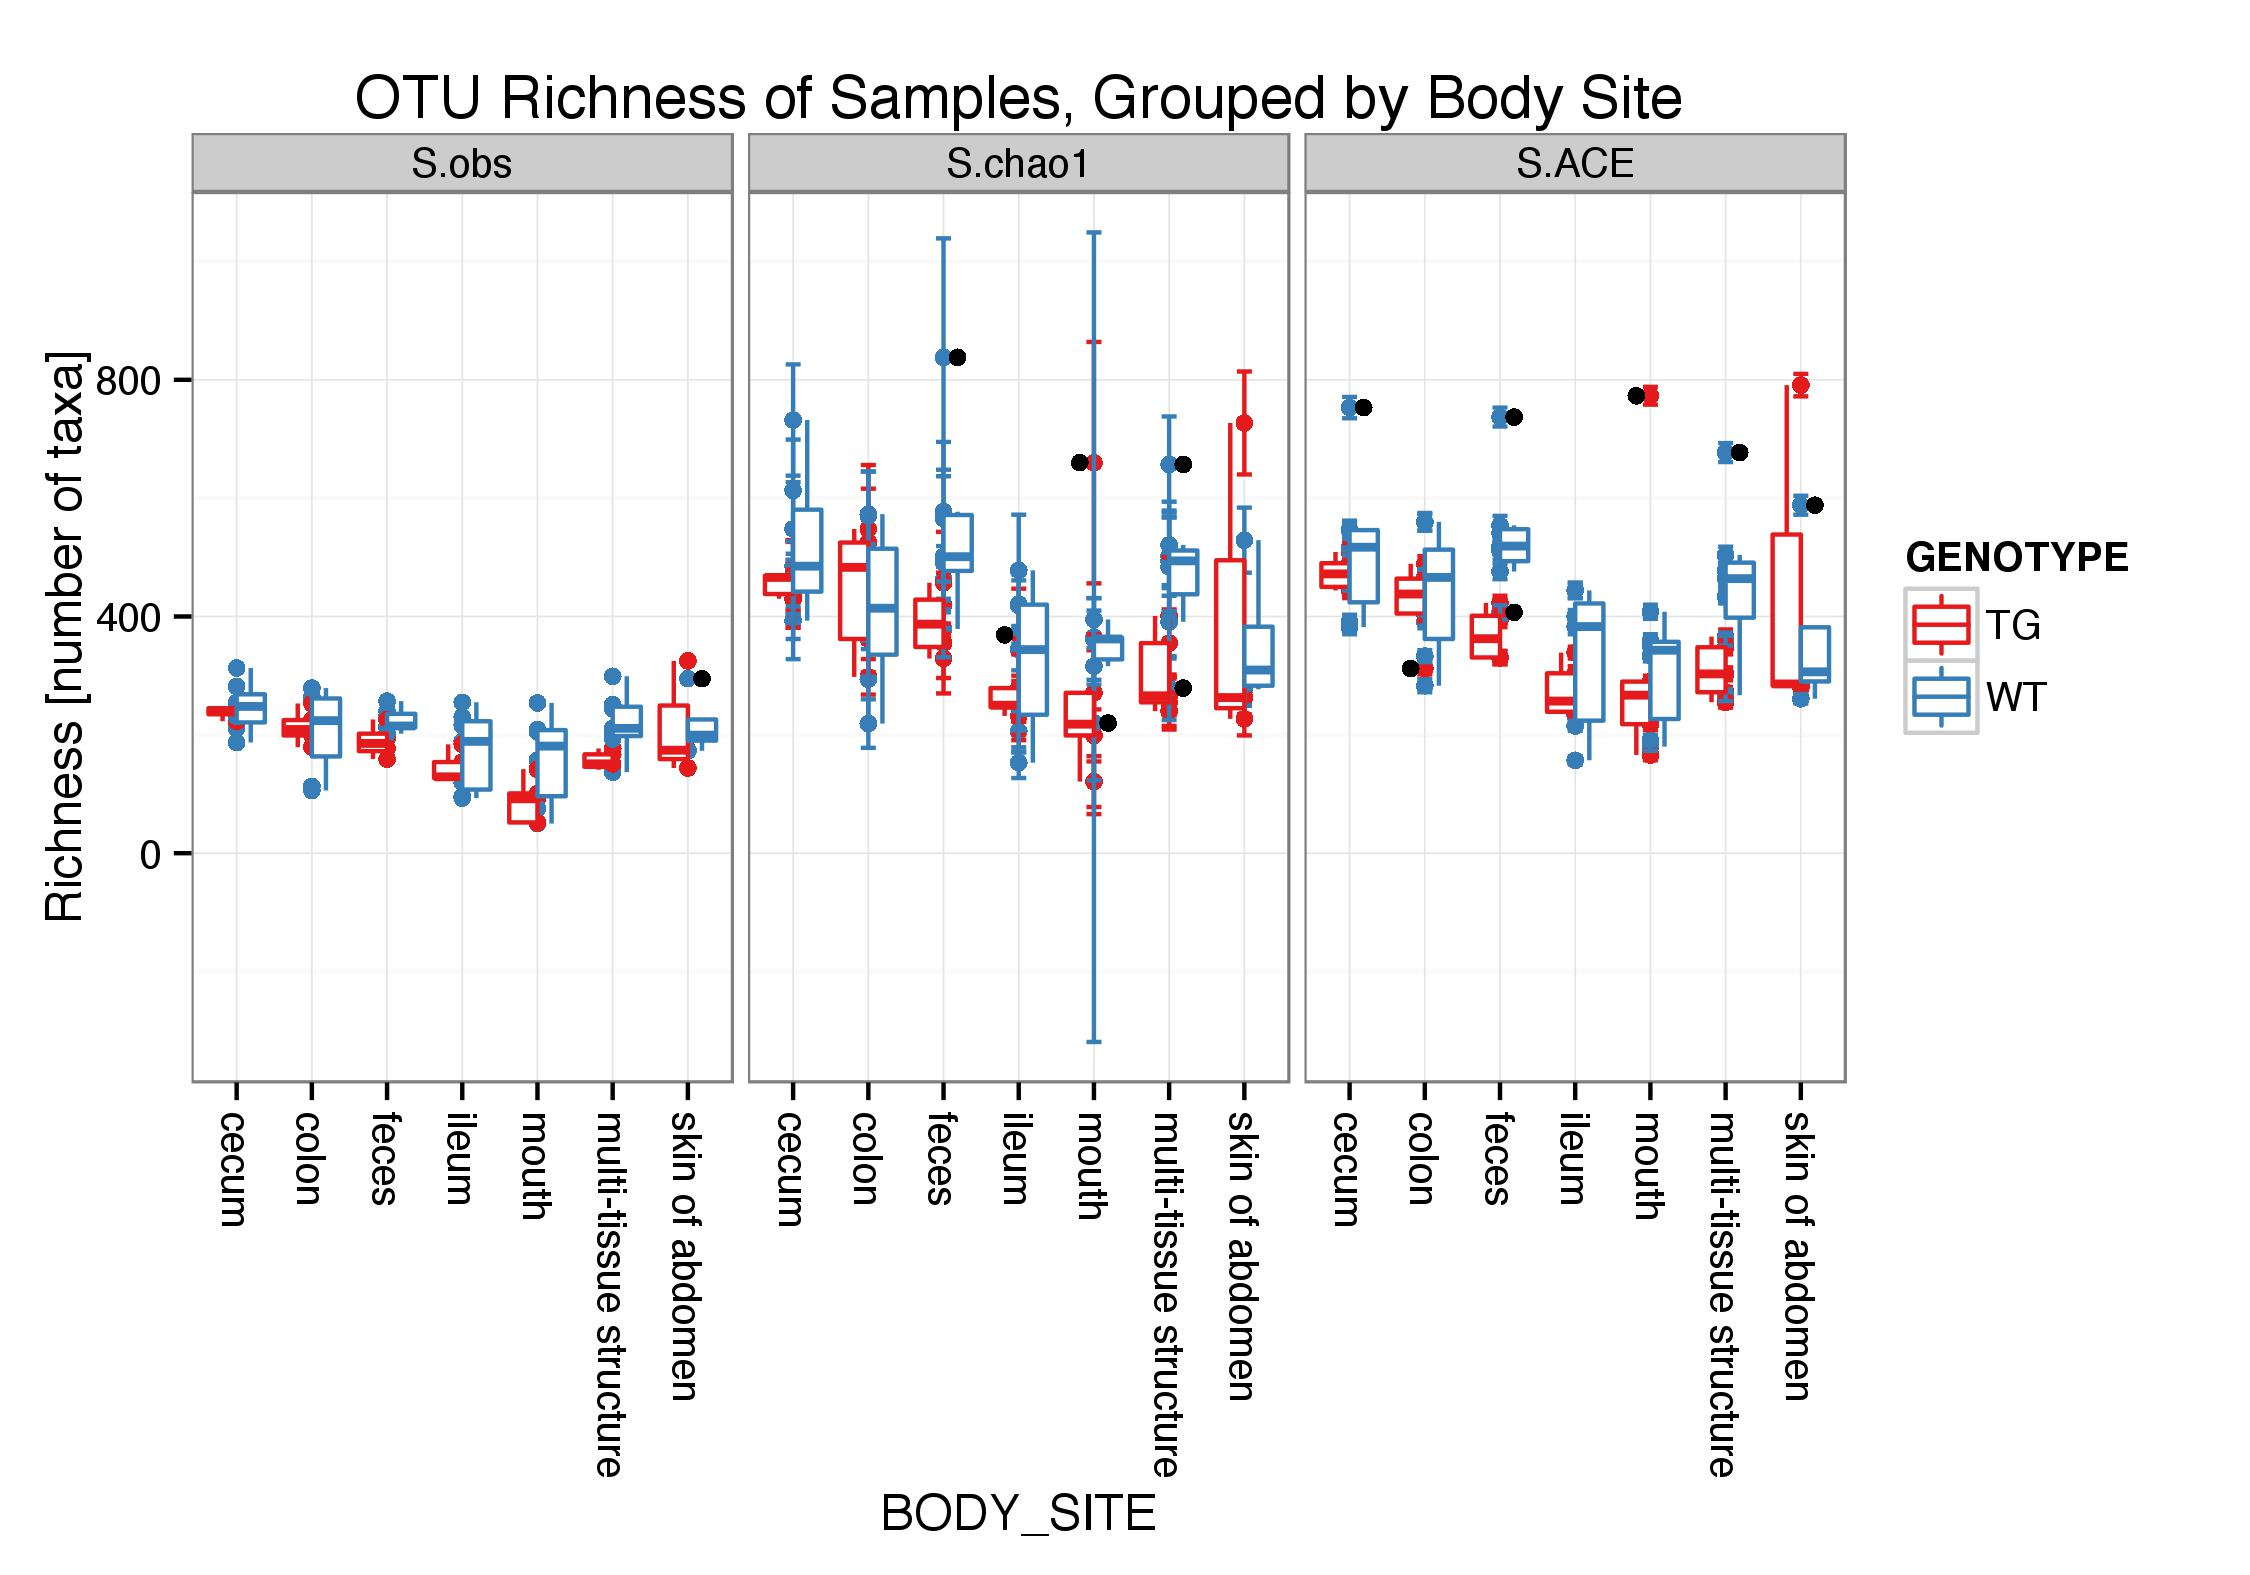
\includegraphics[width=0.75\columnwidth]{chapter_book_figures/Figure_22.jpg}
\caption[Categorically summarized \gls{otu} richness estimates using the plot\_richness function]{\textbf{Categorically summarized \gls{otu} richness estimates using the plot\_richness function.}
Samples are grouped on the horizontal axis according to body site, and color shading
indicates the mouse genotype. The vertical axis indicates the richness estimates in number
of distinct \gls{otu}s, and a separate boxplot is overlaid on the points for each combination
of genotype and body site. The “S.obs”, “S.chao1”, and “S.ACE” panels show the “rarefied”
observed richness, Chao-1 richness, and ACE richness estimates, respectively}
\label{bfigure22}
\end{figure}

\begin{lstlisting}[language=bash]
plot_richness(
  open, x= “BODY_SITE”,
  color = “GENOTYPE”) + geom_boxplot()
\end{lstlisting}

This plot command also illustrates the use of a function in ggplot2, geom\_boxplot,
that instructs the ggplot2 graphics engine to add an additional graphical element –
in this case a boxplot for each of the natural groups in the graphic. These available
additional graphical instructions (called “layers” in the grammar of graphics nomenclature)
are embedded with the returned plot object for subsequent rendering, inspection, or further
modification, allowing for powerfully customized representations of the data.

Here is an example leveraging the abundance bar plot function from phyloseq, plot\_barr,
in order to compare the relative abundances of key phyla between the wild type and
transgenic mice across body sites. The first step was actually some additional data
transformations (not shown, see Supplemental File 1) in order to subset the data to
only major expected phyla (subset\_taxa), merge \gls{otu}s from the same phyla as one entry
(merge\_taxa), and merge samples from the same body site and mouse genotype (merge\_samples).

\begin{lstlisting}[language=bash]
p2 = plot_bar(
  openphyab, “bodysite”,
  fill = “phyla”, title = title)
p2 + facet_gird(∼GENOTYPE)
\end{lstlisting}

From this first bar plot it is clear that all body sites from the average wild type
mouse have Firmicutes as their phylum of largest cumulative proportion, except for the
“feces”, where it is anyway a close call between Firmicutes and Bacteroidetes. By contrast,
some of the average transgenic mice samples have a much higher proportion of Proteobacteria
or Bacteroidetes than the corresponding wild type samples. One drawback to this type of
stacked bar representation is that it is difficult to compare any of the sub-bars except
for those at the bottom. If needed, this can be alleviated by changing the facet\_grid call
such that a separate panel is made for each phyla in the dataset, as follows.

\begin{lstlisting}[language=bash]
p2 + facet_grid(
  phyla ∼ GENOTYPE) + ylim(0, 100)
\end{lstlisting}

With essentially the same effort to produce, the 14 panels of this second bar
plot graphic allow an easy and quantitative comparison of the relative abundances
of each phylum across body sites and genotype.

Microbiome datasets can be highly multivariate in nature, and dimensional reduction
(ordination) methods can be a useful form of exploratory analysis to better understand
some of the largest patterns in the data. Many ordination methods are wrapped in phyloseq
by the ordinate function, and many more are offered in available R packages. Here we
show an example performing multidimensional scaling (MDS) on the precomputed unweighted
UniFrac distance matrix for the open-reference dataset. The ordination result (openUUFMDS)
is first passed to plot\_scree in order to explore the “scree plot” representing the
relative proportions of variability represented by each successive axis. Both
the ordination result and the original data are then passed to plot\_ordination
with sufficient parameters to shade the sample points by genotype, and create
separate panels for each body site.

\begin{lstlisting}[language=bash]
openUUFMDS = ordinate(
 open, “MDS,
 distance = UniFrac[[“unweighted”]][[“open””]])
plot_scree(openUUFMDS, “Unweighted Unifrac MDS”)
plot_ordination(open, openUUFMDS, color = “GENOTYPE”)
+ geom_point(size = 5) + facet_wrap(∼BODY_SITE)
\end{lstlisting}

It appears that a subset of the wild-type samples from all but the mouth and
abdomen-skin body sites cluster toward the left of the plot. This appears to be
the major pattern along the axis that also comprises the greatest proportion of
variability in the dataset. At this stage of analysis it seems worthwhile to try
to identify which \gls{otu} abundances are most different between these groups, and then
perform some formal validation/testing of these differences.

\subsection{Recommendations}
Here, we highlight some of the main aspects to take into account when performing microbial community analysis:

\begin{itemize}
    \item Use the open-reference \gls{otu} picking approach if your data allows it. It
    will reduce the running time and will recover all the diversity in your samples.
    \item Perform an \gls{otu} quality filtering based on abundance, by removing singletons,
    for instance. See \cite{Bokulich2013} for further discussion on how to tune this
    quality filtering and its effects on downstream analysis. Quality filtering is
    critical for obtaining reasonable numbers of \gls{otu}s from a sample.
    \item Consider whether you need to remove specific taxa from your study, such
    chloroplast or host DNA sequences when analyzing microbial datasets.
    \item Remove samples from your study that have low coverage (i.e. low \gls{otu} counts).
    They are likely uninformative and usually indicate low-quality reads.
    \item Rarefy your \gls{otu} table in order to mitigate the differences on the sequencing
    effort, so the downstream diversity analyses won’t be biased by the artificial
    diversity generated due to the difference in sequencing depth.
\end{itemize}

\subsection{Conclusions}
\gls{qiime} is a powerful tool for the analysis of bacterial community allowing researchers
to recapitulate the necessary steps in the processing of sequences from the raw data
to the visualizations and interpretation of the results. Two advantages make \gls{qiime} very
useful: fidelity to the algorithms used, and consistency in the analysis. Fidelity is obtained
because \gls{qiime} wraps existing software, preserving the integrity of the original programs and
algorithms designed, created, and tested by the original authors. Consistency is obtained
because \gls{qiime} can be applied to sequences from different platforms, and once the upstream
process is done; the analysis (downstream) process is the same independent of the sequencing
platform used. These characteristics, together with the fact that \gls{qiime} is open-source software
with continuous support to users via \gls{qiime} forum, have promoted the rapid increase in the \gls{qiime}
user community since its publication \cite{Caporaso2010}.

Downstream and upstream processes are implemented in \gls{qiime} in a way that offers several options
to perform the analyses. In this review, we discuss and demonstrate the principles for each step,
what the scripts do and how to choose between options. Independent of the use of \gls{qiime}, this
review also provides an overview of many of the typical steps in a microbial community analysis
based on analysis of 16S rRNA sequences produced by high-throughput sequencing. Some of these tools
are well developed with a long history in general ecology, whereas others are still in rapid development;
we encourage microbial ecologists and bioinformaticians to work together to create, develop and implement
new strategies and tools that allow further exploration of this fascinating field.

\subsection{Acknowledgments}
We thank William A Walters and Jessica Metcalf for productive discussion and their
useful comments about \gls{qiime}. We also acknowledge Manuel Lladser for helping
collect the dataset and allowing us to use it, and the IQBio IGERT grant for funding
data collection. JANM is supported by a graduate scholarship funded jointly by the Balsells
Foundation and by the University of Colorado at Boulder. SH is partially supported by
NIH grant R01 GM086884. This work was partially supported by the Howard Hughes Medical Institute.
